\documentclass{vldb}
\setlength{\pdfpagewidth}{8.5in}
\setlength{\pdfpageheight}{11in}

\usepackage{graphicx}
\usepackage{balance}  % for  \balance command ON LAST PAGE  (only there!)
\usepackage{subfigure}
\usepackage{enumerate}
%
\usepackage{caption}% in order to have figures without number
\usepackage{wrapfig}
\usepackage{hyphenat}
%\usepackage[labelfont=bf,textfont=bf]{caption}
%\usepackage[utf8]{inputenc}
\usepackage{algorithm}
\usepackage{color} % for colors of MBRs
\usepackage{amsmath}
\usepackage[noend]{algpseudocode}

\newcommand{\hide}[1]{}
\newcommand{\fref}[1]{Figure \ref{#1}}
\newcommand{\sref}[1]{Section \ref{#1}}
\newcommand{\aref}[1]{Algorithm \ref{#1}}
\newcommand{\tref}[1]{Table \ref{#1}}

\newtheorem{theorem}{Theorem}
\newtheorem{lemma}{Lemma}
\newtheorem{remark}{Remark}


\newcommand{\SJ}{TOUCH}
\newcommand{\newSJ}{EVERGREEN}
\newcommand{\dSJ}{dTOUCH}
\newcommand{\cSJ}{cTOUCH}
\newcommand{\reSJ}{reTOUCH}
\newcommand{\rereSJ}{re*TOUCH}

\algnewcommand{\Continue}{\textbf{continue}}%
\algnewcommand{\algorithmicgoto}{\textbf{GOTO line}}%
\algnewcommand{\Goto}[1]{\algorithmicgoto~\ref{#1}}%

\renewcommand{\baselinestretch}{0.97}

\begin{document}

\conferenceinfo{SIGMOD'15,} {May 31- June 4, 2015, Melbourne, Victoria, Australia.}
\CopyrightYear{2015}
\crdata{978-1-4503-2037-5/13/06}
\clubpenalty=10000
\widowpenalty = 10000

\title{reTOUCH: A more workload balanced In-Memory Spatial Join by Iterative Hierarchical Data-Oriented Partitioning}

\hide{
\numberofauthors{3}
\author{
\alignauthor Sadegh Nobari$^\P$$^\dag$
\alignauthor Farhan Tauheed$^\dag$$^\ddag$
\alignauthor Thomas Heinis$^\dag$
\and
\alignauthor Panagiotis Karras$^\S$
\alignauthor St\'{e}phane Bressan$^\P$
\alignauthor Anastasia Ailamaki$^\dag$
\and\affaddr{$^\P$National University of Singapore, Singapore}
\and\affaddr{$^\dag$Data-Intensive Applications and Systems Lab, \'{E}cole Polytechnique F\'{e}d\'{e}rale de Lausanne, Switzerland}
\and\affaddr{$^\ddag$Brain Mind Institute, \'{E}cole Polytechnique F\'{e}d\'{e}rale de Lausanne, Switzerland}
\and\affaddr{$^\S$Department of Management Science and Information Systems, Rutgers University, USA}
}
}

\maketitle

\begin{abstract}
%distance join are important for many applications
Efficient spatial joins are pivotal for many applications and particularly important for geographical information systems or for the simulation sciences
where scientists work with spatial models. Past research has primarily focused on disk-based spatial joins; efficient in-memory approaches, however,
are important for two reasons: a) main memory has grown so large that many datasets fit in it and b) the in-memory join is a very time-consuming part
of all disk-based spatial joins.

In this paper we develop \textbf{TOUCH}, a novel in-memory spatial join algorithm that uses hierarchical data-oriented space partitioning, thereby keeping both
its memory footprint and the number of comparisons low. Our results show that TOUCH outperforms known in-memory spatial-join algorithms as well as in-memory
implementations of disk-based join approaches. In particular, it has a one order of magnitude advantage over the memory-demanding state of the art in terms of
number of comparisons (i.e., pairwise object comparisons), as well as execution time, while it is two orders of magnitude faster when compared to approaches
with a similar memory footprint. Furthermore, TOUCH is more scalable than competing approaches as data density grows.
\end{abstract}

%\terms{Algorithms}
\vspace{-3mm}
% categories
\category{H.2.8}{DATABASE MANAGEMENT}{Spatial databases and GIS}
\category{G.2.2}{DISCRETE MATHEMATICS}{Graph Theory}
\vspace{-2mm}
\keywords{Scalable algorithms; Spatial joins; TOUCH; Indexing}
\vspace{-2mm}
\section{Introduction}
% TODO: make sure we mention unindexed
Many applications dealing with spatial data rely on the efficient execution of spatial or distance joins. In geographical applications these joins are used to
detect collisions or proximity between geographical features~\cite{gis}, i.e., landmarks, houses, roads, etc. and in medical imaging, spatial joins are used to
determine which cancerous cells are within a certain distance of each other~\cite{pais}. In the simulation sciences, where scientists build and simulate precise
spatial models of the phenomena they are studying, distance joins are, for example, used to monitor the folding process of peptides~\cite{peptidefolding}.

Unfortunately, a distance join on two unsorted and unindexed datasets is a computationally costly operation, even if executed in the main memory of a
supercomputer. Data models grow fast and, as a result, the distance join is a bottleneck in many scientific applications today, preventing them from scaling to
bigger models. Apart from growing, data models in real-world scientific applications also become increasingly realistic and hence denser. The growing density of
the models substantially increases the join's selectivity, rendering the efficient execution of this operation key for scaling to larger and more realistic models.

To formulate the problem, we translate the distance join into a spatial join that tests pairs of objects for intersection. Formally, the distance join takes a
distance $\epsilon$ and two spatial datasets $A$ and $B$ and finds all pairs of spatial objects $a \in A$ and $b \in B$ such that the distance between $a$ and
$b$ is less than or equal to $\epsilon$. To translate the problem into a spatial join, we increase the size of all objects in one dataset by $\epsilon$
and then test both datasets for intersecting objects~\cite{spatialjointechniques}.

Existing research on spatial joins has mostly focused on disk-based approaches. Spatial join techniques designed for use in memory hence lack efficiency and
scalability. In this paper we develop TOUCH, a two-way spatial join approach that works efficiently in memory. TOUCH combines concepts from previous work
and avoids their problems, i.e., excessive memory footprint and excessive number of comparisons. In particular, it uses a hierarchy to mitigate replication of
elements and data-oriented partitioning to avoid excessive pairwise comparisons. Additionally, data-oriented partitioning further reduces the number of
comparisons by not considering the objects spatially far from other objects.

Because of the limited work on in-memory spatial joins, we also draw inspiration from on-disk approaches and compare our approach to disk-based approaches used
in memory. The latter is reasonable as growing memory capacities allow for approaches with a bigger memory footprint, originally designed for use on disk, to be
used in main memory.

% the Blue Brain project (BBP)~\cite{bluebrain}
We apply our solution on the "touch detection" problem, a challenging neuroscience application that arises in collaboration with computational
neuroscientists. The neuroscientists build biophysically realistic models with data acquired during anatomical research of the rat brain. In their models, as in
the rat brain, each neuron has branches extending into large parts of the tissue. The neurons receive and send information to other neurons using these
branches. To determine where in the model to place the synapses (structure that permits a neuron to pass a signal to another neuron), it suffices to find the
places where the distance between two branches is below a given threshold~\cite{tabulating}, i.e., where the neurons touch.

Our experiments show that TOUCH outperforms existing spatial joins algorithms in terms of number of comparisons and execution time. When compared to the
fastest related approach TOUCH requires substantially less memory. In the context of our working example, TOUCH performs the spatial join at least one order of
magnitude faster than related work. Our experiments also indicate that TOUCH will scale better to more detailed and denser neuroscience datasets in the future.

Our work has significant potential impact beyond neuroscience applications. Spatial joins are broadly used in many applications beyond neuroscience and the
simulation sciences, and their use in memory is becoming increasingly important in many applications for two reasons. First, main memory has grown so large that
many datasets fit into it directly and the spatial join can be entirely performed in memory. Second, the in-memory join is also an integral part of all
disk-based joins. Disk-based joins partition datasets that do not fit in memory and then join the partitions in memory. Speeding up the in-memory join helps to
considerably speed up on-disk approaches as a whole as well, particularly if the join is very selective and many objects need to be compared (thus spending
a large share of the overall time for the in-memory join).


The remainder of the paper is structured as follows. We discuss related work and its shortcomings in \sref{s_related_work}. In \sref{s_motivation} we motivate
our work and in \sref{s_touch} we present \SJ, our algorithm, and discuss its implementation in \sref{s_implementation}. We compare \SJ~to related approaches in
\sref{s_experimental_evaluation} and draw conclusions in \sref{s_conclusions}.


% The existing algorithms performing spatial join can be divided by the assumption of having index on both, one or none of the datasets. In this paper we propose
% a novel algorithm that assumes having no index on both datasets. Among the many possibilities of having no index on the datasets we can mention the cases when
% creating the index is costly or the datasets are the intermediate results of another process.
\vspace{-3mm}
\section{Related Work}
\label{s_related_work}

\begin{table*}
\centering
\begin{tabular}{ |l|l| }
  \hline
  \multicolumn{2}{|c|}{Terminology table} \\
  \hline
  highest level & level of the root node \\
  lowest level & level of the leaf nodes \\
  higher level & level closer to the highest level \\
  lower level & level closer to the lowest level \\
  A or dataset A or type A or blue& First spatial dataset \\
  B or dataset B or type B or red& Second spatial dataset \\
  $T_A$ & R-Tree created for dataset A \\
  $L_{T_A}$ & Level of the tree $T_A$ \\
  MBR & Minimum Bounding Box (for any dimension) \\
  node's self-mbr & mbr that contains the objects assigned to the node \\
node's light-mbr & contains the leaf level objects below the node\\
node's dark-mbr & contains objects assigned to the descendant nodes excluding leaf nodes below the node\\
nodes's mbr & is union of all the node's mbrs, i.e. light-, dark- and self-mbrs\\
$P^{B}_{T_A}$ & the probability of assigning an object of dataset B to $T_A$ \\
  \hline
\end{tabular}
\caption{Terminologies used in this paper.}
\label{table:terms}
\end{table*}

% TODO: illustrate the mbrs by filled and unfilled boxes and also a figure that shows all the mbr types of a paricular node.

While several spatial join approaches have been developed for disk in the past, only few have been developed for use in memory. Many disk-based spatial join
algorithms, however, can also be used in memory. In the following we discuss all related work no matter if it has traditionally been used for disk or in memory.
\vspace{-1mm}
\subsection{In-Memory Approaches}
Only two approaches have been developed for use in memory and thus have a small memory footprint: the nested loop join~\cite{joinprocessing} and the plane-sweep
join~\cite{computationalgeometry}.


The nested loop join iterates over both spatial datasets in a nested loop and compares all pairs of objects. While this results in a complexity of
$O(n^2)$, no additional data structures are needed, making the approach very space efficient.


The plane-sweep approach sorts the datasets in one dimension and scans both datasets synchronously. All objects on the sweep plane (stored in an efficient data
structure) are compared to each other to see if they overlap. Because the objects are only sorted in one dimension, objects which are not near each other in the
other dimensions may be on the sweep plane at the same time, thus leading to redundant comparisons and hence slowing down the approach.


Despite its deficiencies, however, the plane-sweep approach is still broadly used to join in memory the partitions resulting from disk-based spatial joins.

\vspace{-2mm}
\subsection{On-disk Approaches}
Because they can also be used in memory, in the following we discuss distance join approaches designed for disk. We categorize the approaches based on whether
they require an index on both, one, or none of the datasets.

\vspace{-2mm}
\subsubsection{Both Datasets Indexed}
\label{both}
If both datasets $A$ and $B$ are indexed with R-Trees~\cite{rtree}, a synchronous traversal~\cite{join:RTree} can be used to join them. With the R-Tree indexes
$I_A$ and $I_B$ on datasets $A$ and $B$, this approach starts from the roots of the trees and synchronously traverses the tree to the leaf level. If two nodes
$n_A \in I_A$ and $n_B \in I_B$ on the same level (one from each tree) intersect, then the children of $n_A$ will be tested for intersection with the children
of $n_B$. This process recursively traverses the trees to the leaf level where the objects are compared.

By building on the R-Tree, this approach also inherits the problems of the R-Tree, namely inner node overlap and dead space. Overlap in the R-Tree structure
leads to too many comparisons and hence slows down the join operation. Extensions like the R*-Tree~\cite{rstartree} or the R+-Tree~\cite{rplustree} have been
proposed to reduce overlap. The former tackles overlap with an improved node split algorithm (reinsertion of spatial objects if a node overflows) while the
latter duplicates objects to reduce overlap. Duplicating objects, however, also leads to duplicate results which have to be filtered.

Arguably the most efficient R-Trees can be built through bulkloading if the data is known a priori. Several bulokloading approaches like the STR~\cite{str},
Hilbert~\cite{index:HilbertRTree}, TGS~\cite{tgstree} and the PR-Tree~\cite{prtree} have been developed, all yielding better performance than R+-Tree or
R*-Tree. The R-Tree resulting from bulkloading with Hilbert and STR perform similarly and outperform TGS as well as the PR-Tree on real-world data. TGS and the
PR-Tree, however, outperform STR and Hilbert on data sets with extreme skew and aspect ratio.

Double index traversals are also possible with Quadtrees~\cite{cascadedquadtree} (or Octrees in 3D). Similar to the R+-Tree objects are duplicated (or
references to the objects) and duplicate results are possible and need to be filtered at the end~\cite{hashing}.

\vspace{-2mm}
\subsubsection{One Dataset Indexed}
\label{one}
Extending on a basic nested loop join approach, the indexed nested loop join~\cite{databasefundamentals} requires an index $I_A$ for dataset $A$. The approach
loops over dataset $B$ and queries $I_A$ for every object $b \in B$. Executing a query for each object is a substantial overhead, particularly if $B >> A$.

The seeded tree approach~\cite{join:SeededTree} also requires one dataset to be indexed with an R-Tree. The existing R-Tree $I_A$ on dataset $A$ is used to
bootstrap building the R-Tree $I_B$ on dataset $B$. After building the second index $I_B$, a synchronous traversal~\cite{join:RTree} is used for the join. Using
the structure of $I_A$ to build $I_B$ ensures that the bounding boxes of both indexes are aligned, thereby reducing the number of bounding boxes that need to be
compared. Improvements avoid memory thrashing~\cite{join:SlotIndex} or use sampling to speed up building the R-Tree~\cite{join:Hash}.

\vspace{-2mm}
\subsubsection{Unindexed}
Disk-based approaches first partition both datasets and then join the resulting partitions in-memory. When assigning spatial objects to partitions, some objects
may intersect with several partitions. Two different approaches, \emph{multiple assignment} and \emph{multiple matching}, have been developed to deal with this
ambiguity.

\noindent\textbf{Multiple Assignment:} this strategy assigns each spatial object to all partitions it overlaps with (through duplication). The advantage is that
the distance join only needs to compare objects inside one partition with each other (and not across partitions). Duplication, however, has major drawbacks,
namely a) more comparisons need to be performed and b) because result pairs may be detected twice they need to be deduplicated either at the end (by keeping all
results, thereby increasing the memory used - and deduplicating them at the end) or throughout the join~\cite{deduplication}.

\begin{figure}[htb]
    \begin{center}
        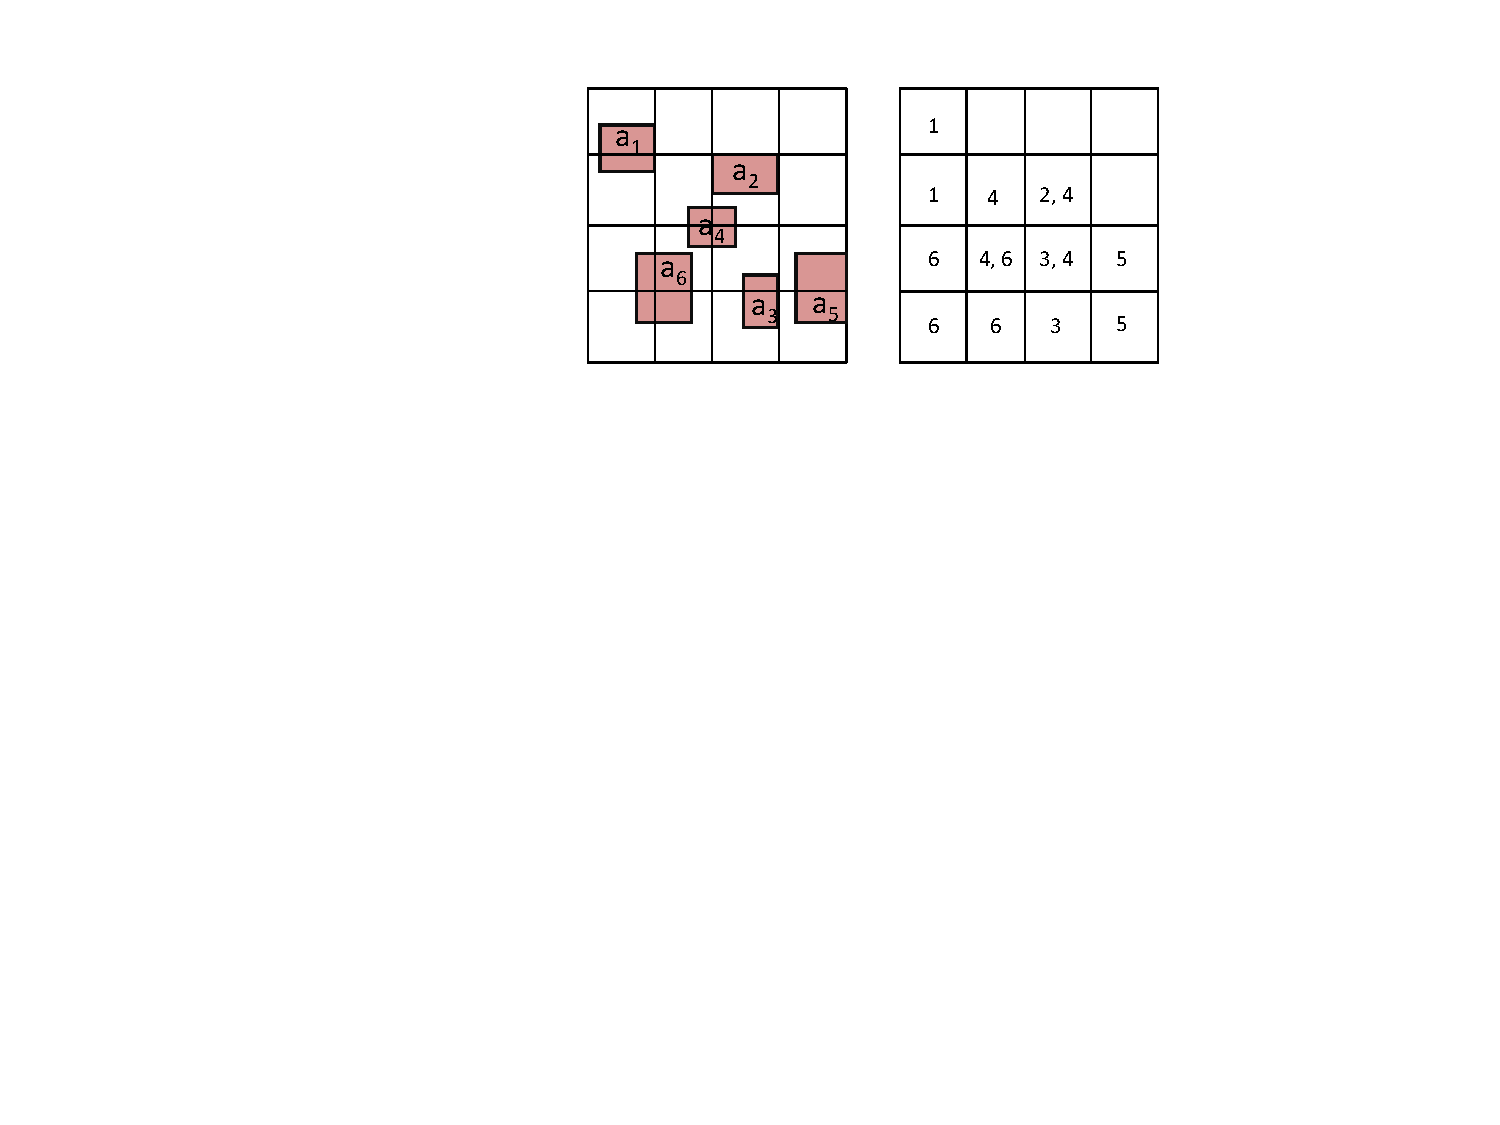
\includegraphics[width=.8\columnwidth]{figures/PBSM}
%       \setlength{\abovecaptionskip}{4pt}
%		\setlength{\belowcaptionskip}{-5mm}
        \vspace{-3mm}
        \caption{PBSM partitioning (left) and assignment (right)}
        \label{fig:PBSM}
      \end{center}
\vspace{-5mm}
\end{figure}


PBSM~\cite{join:PBSM} is the most recent and comparatively most efficient multiple assignment approach. As shown in \fref{fig:PBSM}, PBSM partitions the entire
space of both datasets into cells using a uniform grid. Every object from dataset $A$ is assigned to all cells $c_A$ it overlaps and all $b \in B$ are assigned
to cells $c_B$ respectively. After assigning all objects to cells, all pairs of cells $c_A$ and $c_B$ which have the same position are compared, i.e., all
objects assigned to $c_A$ and $c_B$ are tested for intersection. Because objects are replicated intersections may be detected multiple times and hence
deduplication needs to be performed.


The non-blocking parallel spatial join NBPS~\cite{join:nonblocking} algorithm produces the result tuples continuously as they are generated. NBPS distributes the tuples of the join relations to the data server nodes according to a spatial partitioning function. In contrast to PBSM, NBPS avoids duplicates so that the result can  be returned immediately. More precisely, NBPS uses a revised reference point method to avoid the duplicates while TOUCH uses a hierarchical partitioning that not only avoids any replication (in comparison with NBPS) but also avoids the duplicates from the first stage of the distribution.

%Luo et. al. in \cite{join:nonblocking} proposes a non-blocking parallel spatial join (NBPS) algorithm which produces the resulted tuples continuously as they are generated. NBPS distributes the tuples of the join relations to the data server nodes according to a spatial partitioning function. In contrast to the PBSM algorithm, NBPS uses a duplicate avoidance techniques in order to output the results immediately. However, NBPS uses a revised reference point method to avoid the duplicates while TOUCH uses a hierarchical partitioning that not only avoids any replication (in comparison to NBPS) but also avoids the duplicates from the first stage of the distribution.

% throughout the join~\cite{deduplication} or at the end (all unique results are kept and deduplicated before the end).

\noindent\textbf{Multiple Matching:} this strategy on the other hand assigns each spatial object only to one of the partitions it overlaps with. Hence when
joining, objects in several partitions must be compared with each other, as an object at the border of one partition can potentially intersect with an object at
the border of an adjacent partition.

The Scalable Sweeping-Based Spatial Join~\cite{sssj} is similar to PBSM but avoids replication. It partitions space into $n$ equi-width strips in one dimension
and maintains for every strip two sets $LA_n$ and $LB_n$. It assigns each $a \in A$ that entirely fits into strip $n$ to $LA_n$ and for $B$ and $LB_n$
respectively. Finally, it uses an in-memory plane-sweep to find all intersecting pairs from $LA_n$ and $LB_n$ for all $n$.

An object $o$ intersecting several strips will not be replicated but will instead be assigned to sets $LA_{jk}$ and $LB_{jk}$ respectively where $j$ is the
strip where $o$ starts and $k$ where $o$ ends. When joining $LA_n$ and $LB_n$ all sets $LA_{jk}$ and $LB_{jk}$ with $j \le n \le k$ will also be considered in the
plane-sweep.

% For this approach to work, both sets $LA_n$ and $LB_n$ of a strip $n$ need to be loaded entirely into memory. If this is not possible both sets $LA_n$ and
% $LB_n$ will be recursively partitioned into several strips again.


\begin{figure}[htb]
    \begin{center}
        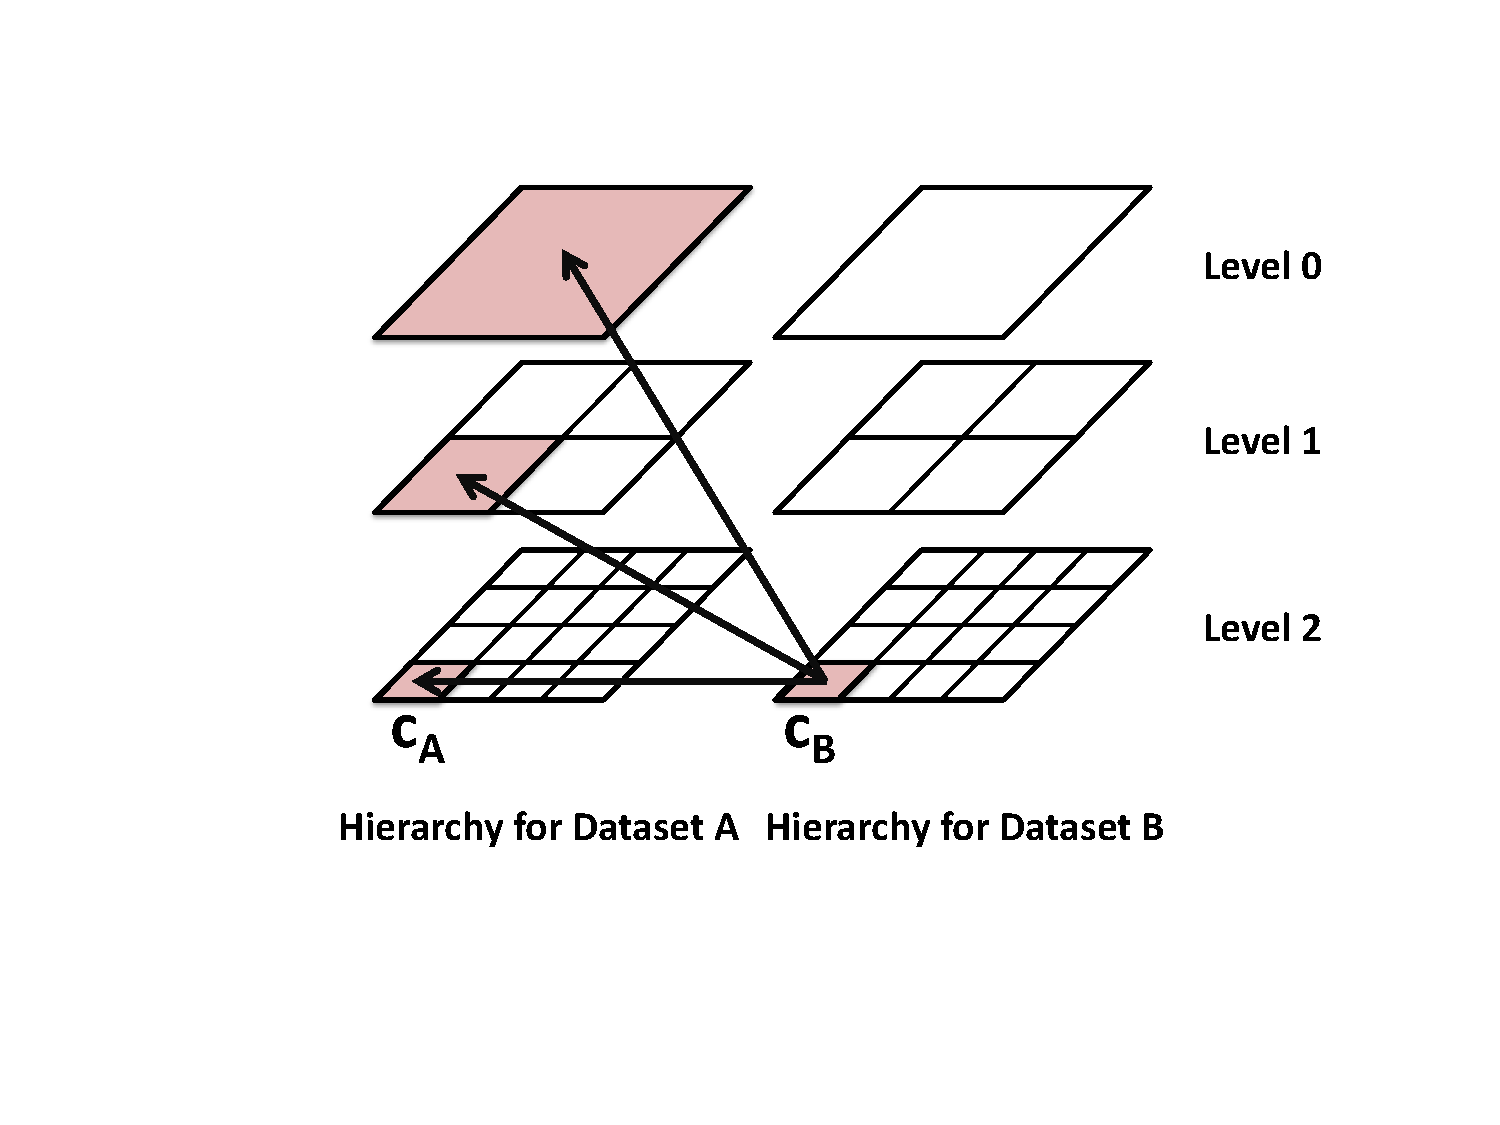
\includegraphics[width=.8\columnwidth]{figures/SizeSeparation}
%        \setlength{\abovecaptionskip}{4pt}
%		\setlength{\belowcaptionskip}{-5mm}
\vspace{-3mm}
        \caption{S3 space partitioning and multi-level join.}
        \label{fig:SizeSeparation}
      \end{center}
\vspace{-9mm}
\end{figure}

To avoid the replication of objects, S3~\cite{join:SizeSeparation} maintains a hierarchy of $L$ equi-width grids of increasing granularity as shown in
\fref{fig:SizeSeparation}. In $D$ dimensions the grid on a particular level $l$ has $(2^l)^D$ grid cells and assigns each object of both datasets to a grid cell
in the lowest level where it only overlaps one cell. To obtain this assignment, the algorithm starts with level L (Level 2 in figure 2) and moves up the levels until it finds the
level where the object only overlaps one cell.

The algorithm maintains two hierarchies, $H_A$ for dataset $A$ and $H_B$ for dataset $B$. Once all objects are assigned, the cells of $H_A$ and $H_B$ are
joined. More precisely, a cell $c_B$ of $H_B$ is joined with its corresponding cell $c_A$ of $H_A$ and all the cells on higher levels of $H_A$ enclosing $c_A$
(example cells are shaded in \fref{fig:SizeSeparation}). Joining a cell with its counterpart as well as with cells on higher levels is repeated on all levels.

The process of joining the cells implies that the objects assigned to the highest level will be compared to all other objects (on all lower levels) and hence
the more objects are assigned to the highest level, the more comparisons will be needed. Datasets assigning more objects to levels closer to the leaf level will
require fewer comparisons for the join.


\section{Challenge}
\label{s_motivation}
The development of \SJ~is driven by the requirements of the computational neuroscientists we collaborate with. In order to better understand how the brain
works, the neuroscientists build biophysically realistic models of a neocortical column on the molecular level and simulate them on a BlueGene/P with 16K CPUs.
Each of the models contains several thousand neurons where each neuron and its branches are modeled as thousands of cylinders. \fref{f_representation} shows a
cell morphology, with cylinders modeling the dendrite and axon branches in three dimensions.

\begin{figure}[h!]
  \begin{center}
      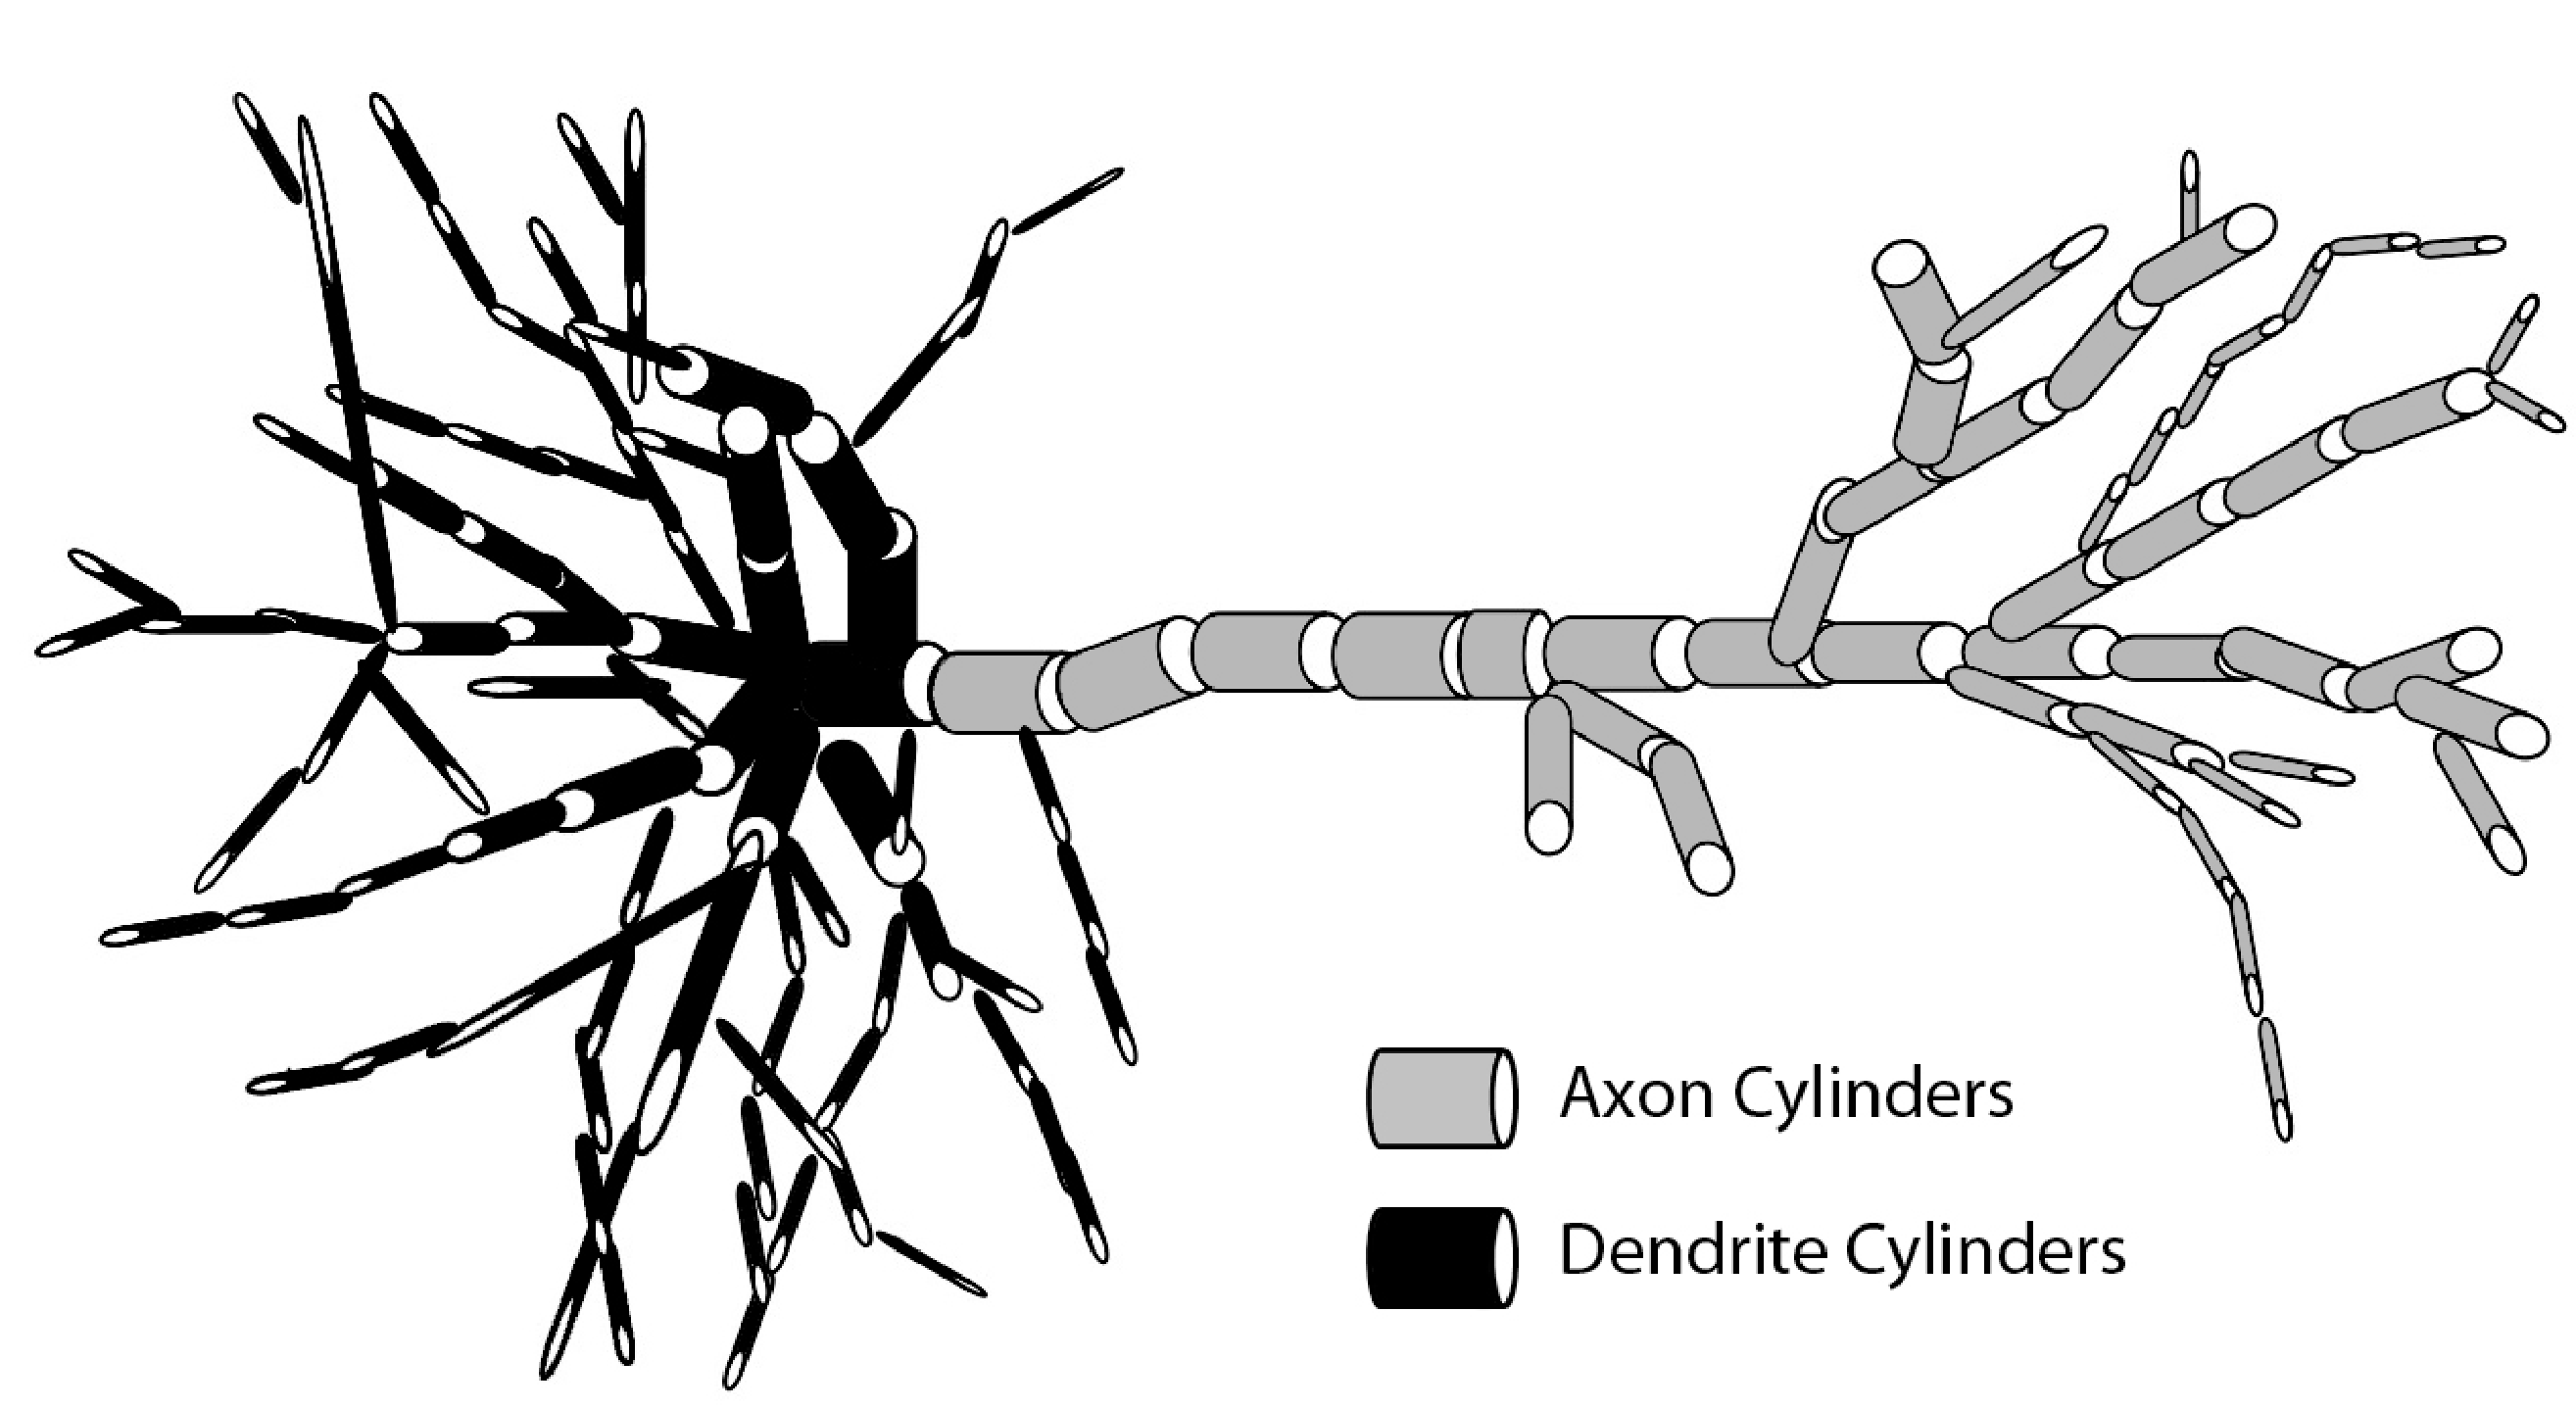
\includegraphics[angle=0, width=0.45\textwidth]{figures/neuron}
%		\setlength{\abovecaptionskip}{4pt}
%		\setlength{\belowcaptionskip}{-5mm}
\vspace{-3mm}
		\caption{Neuron modeled with cylinders.}
      \label{f_representation}
  \end{center}
\vspace{-5mm}
\end{figure}


The models are built based on the analysis of real rat brain tissue. The structure of the neuron is rebuilt using brightfield microscopy and their
electrophysiological properties are obtained by the patch clamp technique~\cite{patchclamp}. The locations of synapses (i.e., points where impulses leap over
between neurons), however, are not known, cannot be determined by the above techniques and thus need to be added in a post-processing step. Placing the synapses
is a one-off operation executed only once for each model built. The synapse locations are determined by the following rule: a synapse is placed wherever a
neuron's dendrite is within a certain distance of another neuron's axon. Previous neuroscience research has confirmed that a realistic model of the brain is
built by following this rule~\cite{tabulating}.


The problem of placing synapses therefore translates to a spatial distance join between two unindexed and unsorted datasets, one dataset containing cylinders
representing axons and one containing cylinders representing dendrites. The distance join is only executed once on each new model and thus no data structures
can be shared between distance joins on different models. Because the 16K cores of the BlueGene/P cannot access the disk concurrently, the join has to be
performed in memory alone. Furthermore, this independency is advantageous for data-parallel algorithms that can be executed on GPUs \cite{nobariGPU}.  To do so, and because this is an embarrassingly parallel problem, the dataset is split into 16K contiguous subsets, each subset is
loaded in the memory of a core and the distance join is performed locally (independent of the other cores and thus massively parallel).


% scalability
The models currently built and simulated by the neuroscientists contain at most few million neurons, but the ultimate goal is to simulate the human brain with
approximately $10^{11}$ neurons. To achieve this goal, the number of neurons needs to increase until the model has the same neuron and synapse density as the
human brain. The higher density of a dataset modeling the human brain, as opposed to those modeling the rat brain, will substantially increase the selectivity
of the distance join between the two datasets, as more synapses are found in the former than in the latter. An efficient distance join approach is therefore
pivotal already today and the advancement of neuroscience research requires an in-memory spatial join that will scale to the increasingly high selectivity of
arising models of the brain/neuroscience datasets.

The particular application notwithstanding, an efficient in-memory spatial join is important for many applications: after all, every disk-based spatial
join needs to perform an in-memory join.



\section{\SJ}
\label{s_touch}
Given the lack of adequate in-memory spatial join approaches we develop {\SJ}, a new in-memory spatial join algorithm for two unsorted and unindexed spatial
datasets, $DS_1$ and $DS_2$. We translate the distance join required by our motivating example into a spatial join that detects intersection between objects:
instead of finding all pairs of objects $d_1 \in DS_1$ and $d_2 \in DS_2$ such that $distance(d_1, d_2) \leq \epsilon$, we increase the size of all objects of
one dataset, say $DS_1$, by $\epsilon$ and test for intersection with objects of $DS_2$~\cite{spatialjointechniques}.


\begin{figure}[htb]
    \centering
        \subfigure[The datasets $A$ and $B$]{\centering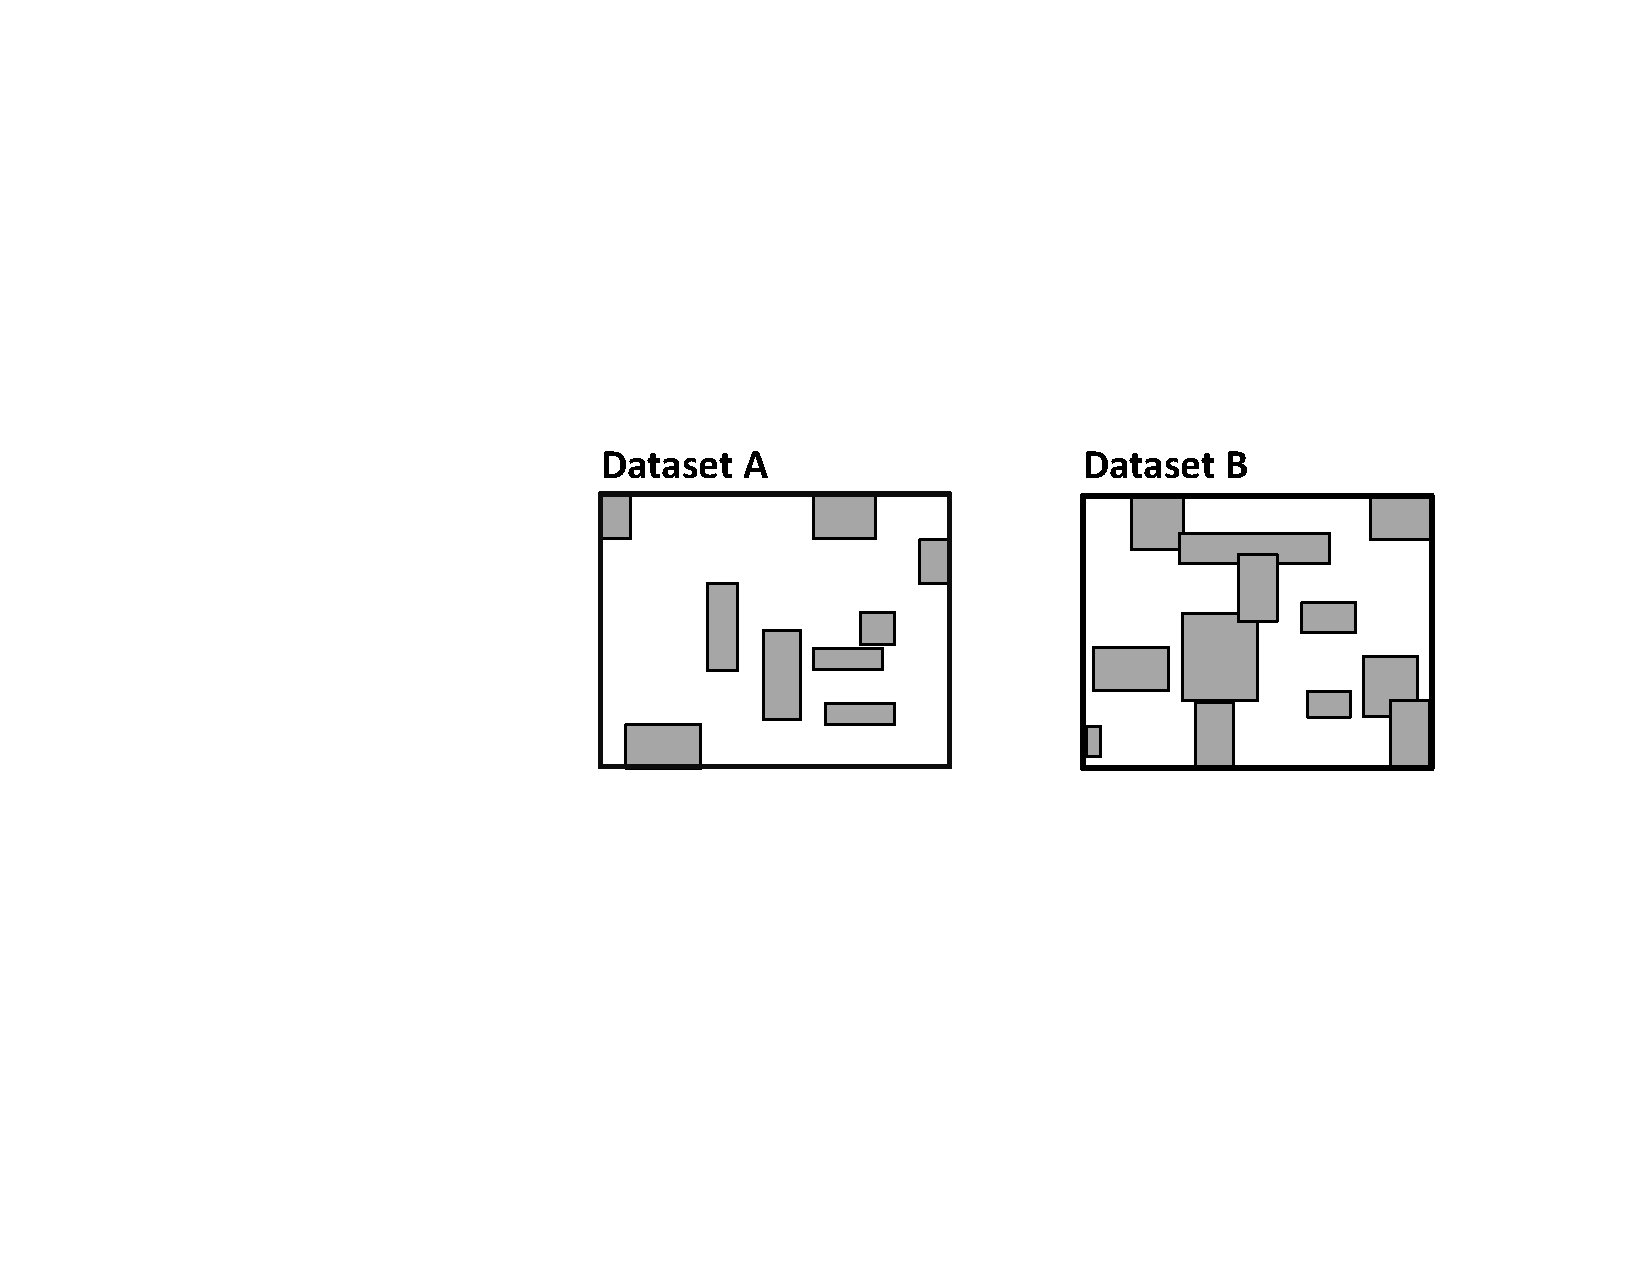
\includegraphics[width=\columnwidth]{figures/TOUCH1}}
        \subfigure[Tree building, assignment and joining phases]{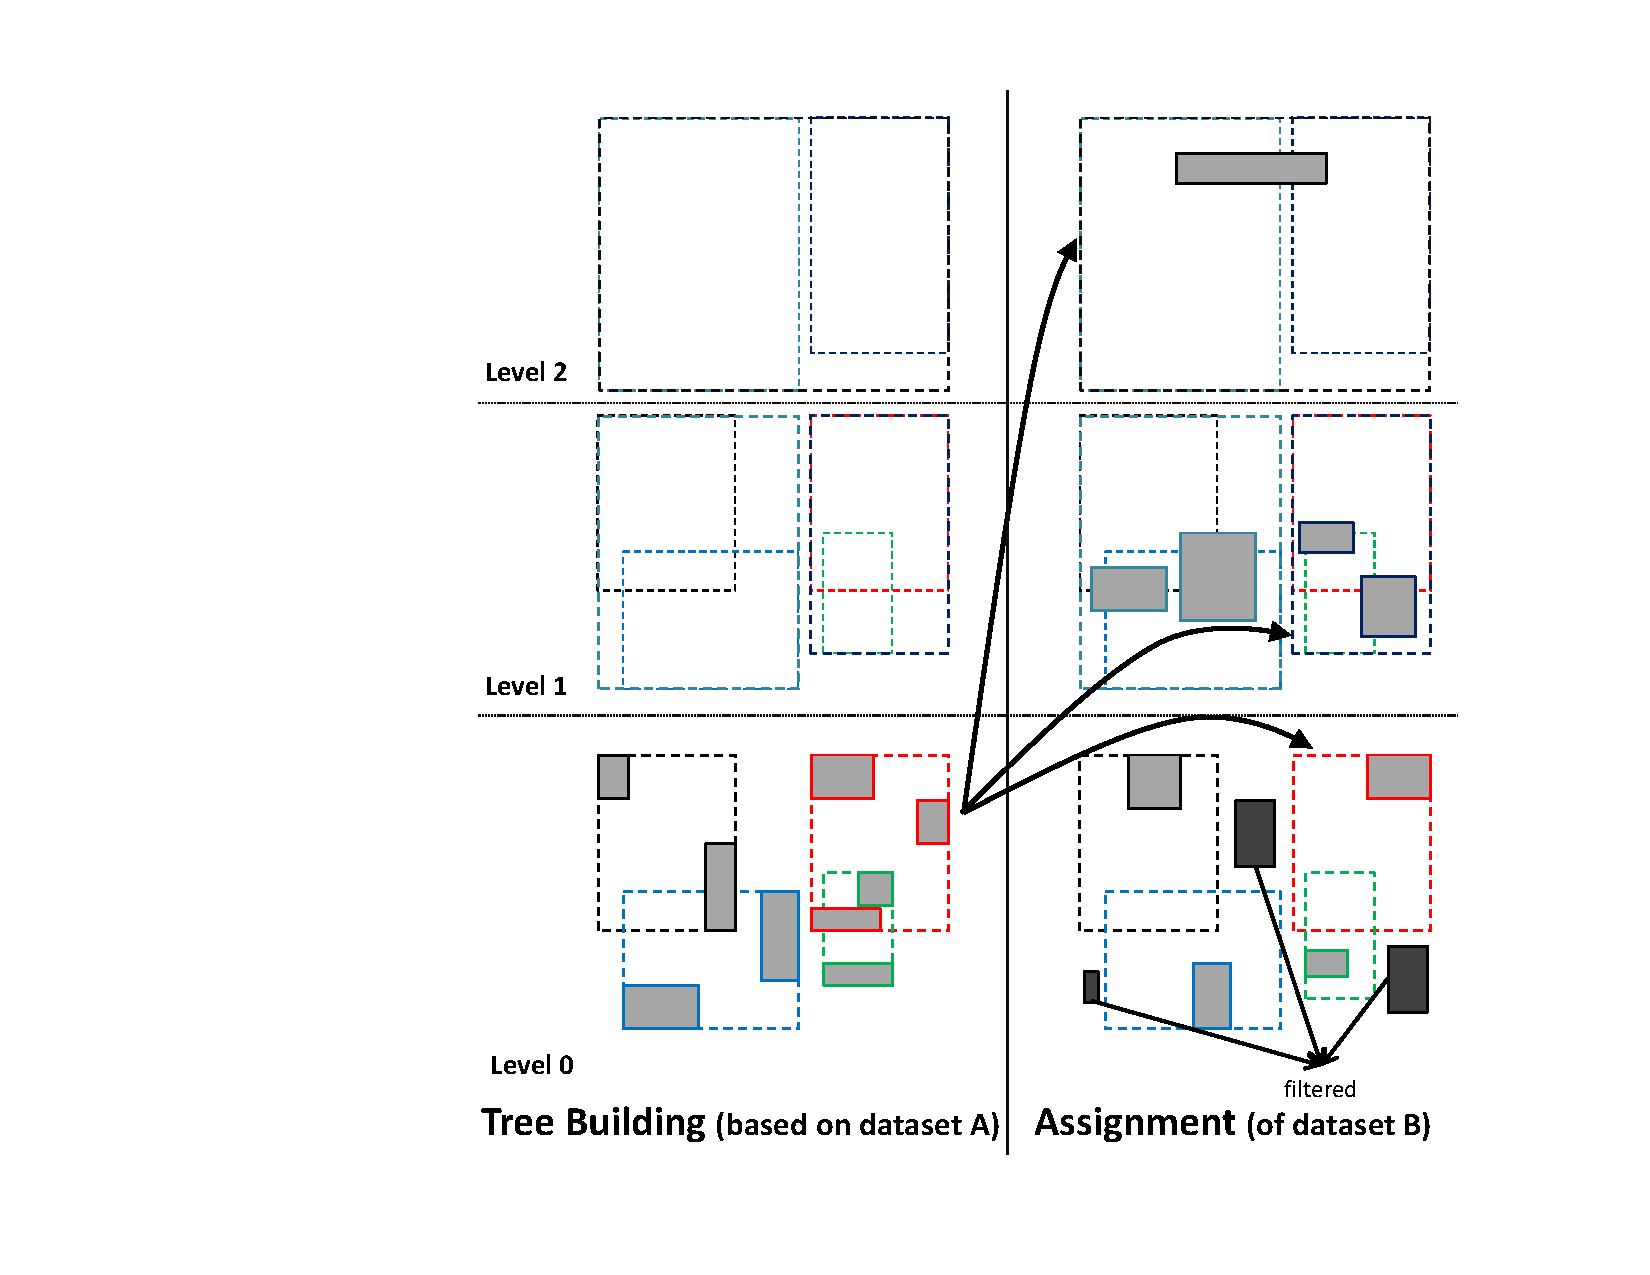
\includegraphics[width=\columnwidth]{figures/TOUCH2}}
%        \setlength{\abovecaptionskip}{4pt}
%		\setlength{\belowcaptionskip}{-5mm}
\vspace{-3mm}
        \caption{The three phases of \SJ: building the tree, assignment and joining.}
        \label{fig:TOUCH}
\vspace{-1mm}
\end{figure}


It is established practice to perform a spatial join in two phases: filtering followed by refinement~\cite{twophasejoin}. Like most other approaches, TOUCH
focuses on the filtering phase in which all objects are approximated by bounding boxes. Our solution can be combined with any off-the-shelf solution to
the second refinement phase, which takes into account the exact object shapes (e.g., cylinders, spheres, etc.).

\subsection{{\newSJ} Ideas}

Big data processing calls for exploiting the ubiquitous parallel processors, e.g. GPU and CPU. These architectures are well designed for independent balanced workloads. Thanks to the {\SJ} algorithm, the workloads are independent. However, we need balanced workloads as well. The reTOUCH algorithms are designed with the idea of creating balanced workload by reducing the asymmetry of the TOUCH algorithms as much as possible. The algorithms are explained in section \sref{s_retouch} in detail.
The followings are the {\SJ} ideas:

In developing \SJ, we are inspired from previous disk-based approaches, which can also be used in main memory. However, we aim to combine the benefits and avoid
the pitfalls of previous approaches. In particular, we want to avoid multiple assignment (as in PBSM), because it replicates objects and therefore (a) increases
the memory footprint; (b) requires multiple comparisons; and (c) makes it necessary to deduplicate the results.

At the same time we want to reduce the number of comparisons of multiple matching approaches and we therefore want to use data-oriented partitioning instead of
space\hyp{}oriented partitioning as S3 does.

To further reduce the number of comparisons, we also use filtering, a concept used by S3. In S3, objects from the second dataset $B$ are discarded if they
intersect only with cells that contain no objects from dataset $A$. If object $b \in B$ is only overlapping cells that contain no object from $A$ then $b$
cannot possibly intersect with any object from $A$. Hence $b$ does not need to be considered further.

The main innovation of TOUCH lies in the fact that it directly assigns objects of the second data set to the data-oriented index of the first. By doing so it
avoids the problems caused by excessive index-overlap in other data-oriented approaches (R-Tree) as well as the problems of space-oriented indexing approaches
(like S3). As we will explain, the combination of data-oriented partitioning during index-building on the first dataset with hierarchical assignment of the
second dataset leads to significantly fewer comparisons and speeds up the join itself.

The fact that we design our approach for use in memory gives us more degrees of freedom. We no longer have to align the data structures for the disk page size,
but can choose the size of the data structures used more flexibly (partitions of arbitrary size, variable fanout, etc.).



\subsection{Proof of Correctness}
We may want to have a similar subsection for reTOUCH algorithms
\hide{
The correctness of \SJ~is proven in Theorem \ref{Theorem:correct}. Lemma \ref{Lemma:NoDup} proves that the result pairs generated by \SJ~(until joining the
buckets, i.e. the global join) are unique. Without loss of generality, in the following we assume that a pair of objects $(a,b)$, $a \in A$ and $b \in B$, is in
the result pairs iff MBR of object $a$ overlaps the MBR of object $b$. In the case of a distance join with a distance of $\epsilon$, we can extend the objects
of a dataset by $\epsilon$ then check the overlapping of the objects in the join.

\vspace{-2mm}
\begin{lemma}[Completeness]
\label{Lemma:complete}
The assignment phase of \SJ~does not miss any pair of overlapping objects.
\end{lemma}
\vspace{-2mm}
\begin{proof}
Assume that object $a$ of dataset $A$ overlaps object $b$ of dataset $B$ and the pair $(a,b)$ is not in the result set of \SJ. Because in the probing phase of
\SJ, $a$ is compared against the bucket it overlaps at each level, and $b$ overlaps with $a$, then $b$ must be inside at least one of these buckets. As a
result, $b$ must be compared against $a$ when $a$'s bucket is joined against the bucket that $b$ is assigned to.
\vspace{-2mm}
\end{proof}

\vspace{-2mm}
\begin{lemma}[Soundness]
\label{Lemma:sound}
The set of result pairs generated by \SJ~is a subset of pairs of overlapping objects.
\vspace{-2mm}
\end{lemma}


\begin{proof}
When a pair of objects $(a,b)$, $a \in A$ and $b \in B$, is not overlapping, then two scenarios are possible. First, the buckets $a$ and $b$ are assigned to
are not overlapping, hence the buckets are not joined with each other. The other possible scenario is that the buckets $a$ and $b$ are assigned to are
overlapping. As a result, the objects inside the buckets are joined with each other. However, because $(a,b)$ are not overlapping, this pair of objects is not
reported as result. Any pair in the set of result pairs of \SJ~hence overlap.
\end{proof}

\vspace{-2mm}
\begin{theorem}\label{Theorem:correct}
\SJ~finds all object pairs that overlap.
\end{theorem}
\vspace{-2mm}
\begin{proof}
The proof follows from Lemmas~\ref{Lemma:complete} and~\ref{Lemma:sound}.
\end{proof}
\vspace{-2mm}
\begin{lemma}[No duplication]\label{Lemma:NoDup}
The set of result pairs generated by \SJ~(until joining the buckets, i.e. the global join) contains unique pairs of objects.
\end{lemma}
\vspace{-2mm}
\begin{proof}
Because each object $b$ of the dataset $B$ is assigned to at most one bucket (single assignment) closest to the leaf level that covers the
object, $b$ is compared against each object of dataset $A$ at most once. Hence, for any $b$, any result pair that contains $b$ appears only once.
\end{proof}
}

\section{{\newSJ} algorithms}
\label{s_retouch}

In this section, we are devising our novel algorithms, called {\dSJ}, {\cSJ}, {\reSJ} and ultimately {\rereSJ} algorithm. Since we are dealing with big data, we need to exploit the ubiquitous parallel processors, e.g. GPU and CPU. These architectures are well designed for independent balanced workloads. Thanks to the {\SJ} algorithm, the workloads are independent. However, we need balanced workloads as well. The {\newSJ} algorithms are designed with the idea of creating balanced workload by reducing the asymmetry of the {\SJ} algorithms as much as possible. These algorithms create indexes that produce even workloads for the actual job. Each of the following designs has pros and cons that worth studying.

In order to explain the {\newSJ} algorithms we need to have an overview of the {\SJ} algorithm. Therefore, next subsection briefly explains the {\SJ} algorithm and the subsequent subsections explain our novel algorithms. For clarity, we assume that the lowest level of a tree is the leaf level and the highest level is the level of root node and accordingly lower and higher levels can be defined. Please find table \ref{table:terms} the list of terminologies used in this paper.

\subsection{Detail information}
We have light, dark, self-dark and black mbrs. black mbr is union of all the other mbrs. light mbr contains the leaf level objects. dark mbr contain assigned object in my descendants and not leaf. self-dark only assigned objects to the node. light mbr is used for faster shrinking after assignment of all the objects of a type of a leaf node. black mbr for the faster assignment. self-dark and dark for those objects that cannot be filtered because they had some overlap on the ancestors assigned objects.


SGH: case 1 and 4.
\begin{itemize}
\item Case 1: Each node joining with descendants' grids on demand.
\item Case 2: Each node joining with ancestors' grids on demand.
\item Case 3: Each node lets descendants join with its own grid.
\item Case 4: Each node lets ancestors join with its own grid.
\end{itemize}


\begin{table}
\centering
\begin{tabular}{ r|c|c| }
\multicolumn{1}{r}{} & Grid at Descendant & \multicolumn{1}{c}{Grid at Ancestor} \\
\cline{2-3}
Top-Down & Case 1 & Case 3 \\
\cline{1-3}
Bottom-Up & Case 4 & Case 2 \\
\cline{2-3}
\end{tabular}
\caption{Tree traversal and grid placement of SGH join.}
\label{table:SGH}
\end{table}


Grid size: every node has an MBR that contains all the objects assigned to the node. For each node we divide each dimension of its MBR to $\sqrt[D]{\frac{|MBR|}{|AVE|}}$ partitions, such that $D$ is number of dimensions, $|MBR|$ is the size of the MBR and $|AVE|$ is the average size of the objects inside the node.

\subsection{{\SJ} algorithm}
The {\SJ} algorithm consists of three steps: Tree construction (Algorithm \ref{alg:touchtree}), Assignment (Algorithm \ref{alg:touchassign}) and Joining (Algorithm \ref{alg:touchjoin}) steps. The algorithms \ref{alg:touchtree}, \ref{alg:touchassign} and \ref{alg:touchjoin} describes the {\SJ} algorithm in a way that smooths our {\newSJ} algorithms explantions that follows subsequently.

\begin{algorithm}
\caption{TOUCH algorithm, building $T_A$}\label{alg:touchtree}
\begin{algorithmic}[1]
\Function{TreeConstruction}{$dataset$}\Comment{$dataset_A$}
\State{$nextInput = (dataset, level=0)$}
\While{$nextInput$ is not empty}
  \State{$(ds, level) = nextInput$}
  \State{SpatialSort($ds$)}\Comment{e.g. Hilber Sort}
   \If{$level=0$}
	  \State{split $ds$ into $partitions$ of size $leafSize$.}
	  \Else
	  \State{split $ds$ into $fanout$ number of $partitions$.}
  \EndIf
    \ForAll{$part \in partitions$}
      \State{$MBR=$ calculate the mininum bounding rectangle that covers all the objects inside $part$.}
      \State{$tree \gets [part, level]$}
      \State{$nextInput \gets$ $(MBR, level = level+1)$}
    \EndFor
\EndWhile
\EndFunction
\end{algorithmic}
\end{algorithm}

Algorithm \ref{alg:touchtree} builds an R-Tree from the objects of $dataset_A$, i.e. $T_A$. This algorithm first partitions the objects by using Hilbert Sort. Then constuct a tree from the created partitions in which each node contains an MBR that covers all the objects in its descendant nodes.

\begin{algorithm}
\caption{TOUCH algorithm, Assignment step}\label{alg:touchassign}
\begin{algorithmic}[1]
\Function{assignment}{$dataset_B$}
\ForAll{$b$ in $dataset_B$\label{alg:assign:loopoverobj}}
    \State{$currentNode =$ root node of $T_A$}
    \State{$S=$ set of nodes $\in$ children of $currentNode$ that $b$ intersects\label{alg:assign:loopoverchilds}}
    \If{$|S|=0$}\Comment{$b$ is filtered}
      \State{\Continue}
    \EndIf
    \If{$|S|=1$}\Comment{go one level lower in $T_A$}
	  \State{$currentNode$ = $S$}
	  \If{$currentNode$ is a leaf node}
	  \State{assign $b$ to $currentNode$ and \Continue}
	  \Else
	  \State{\Goto{alg:assign:loopoverchilds}}
	  \EndIf
	\EndIf\label{alg:assign:assigns}
	\If{$|S|>1$}\Comment{assign to this level}
	  \State{assign $b$ to $currentNode$ and \Continue}
	\EndIf
\EndFor
\EndFunction
\end{algorithmic}
\end{algorithm}

Algorithm \ref{alg:touchassign} assigns the objects of $dataset_B$ to the internal nodes of the constructed tree of the algorithm \ref{alg:touchtree}, $T_A$. The goal of algorithm \ref{alg:touchassign} is to do a \emph{complete assignment} (defined in theorem \ref{Theorem:correctAssignment}) of the objects to the lowest internal node of $T_A$.

\begin{theorem}\label{Theorem:correctAssignment}
An assignment of an object $o$ to an internal node $n$ is complete iff among all the siblings of node %n%, only the MBR of $n$ has overlap with $o$.
\end{theorem}
\begin{proof}
The assignment is complete because neither the siblings nor the ancestors of node $n$ has an object that overlaps with $o$
\end{proof}


\begin{algorithm}
\caption{TOUCH algorithm, Join step}\label{alg:touchjoin}
\begin{algorithmic}[1]
\Function{TJoin}{$treeNode$}\Comment{root node of $T_A$}
\State{$O_B=$ objects of $dataset_B$ assigned to the $treeNode$}
\State{$MBR=$ MBR of $treeNode$}
\State{$gridHash=$ Divide the $MBR$ of $treeNode$ to grid cells with the given $resolution$}
  \ForAll{objects $O_A$ of $dataset_A \in$ descendant leaf nodes of $treeNode$}
	\State{SGH($O_A$, $gridHash$)}
	\Comment{Spatial Grid Hash join}
  \EndFor
  \ForAll{$childNode \in treeNode$}
  \State{TJoin($childNode$)}
  \EndFor
\EndFunction
\end{algorithmic}
\end{algorithm}

Algorithm \ref{alg:touchjoin} performs the required pairwise comparisons according to the assignment of the objects of $dataset_B$ to the $T_A$. The algorithm employs the Spatial Grid Hash join (SGH) for joining the objects of $dataset_B$ in each internal node of $T_A$ with the objects of $dataset_A$ in its (the internal node) descendant leaf nodes. The algorithm starts by traversing $T_A$ top-down. When visiting a node, to perform SGH, the algorithm constructs the grid for the visited node and the objects in its descendants probe the grid. Succinctly, each node lets descendants join with its own grid.


\subsection{{\dSJ} algorithm (double {\SJ})}

\begin{figure}[htb]
    \begin{center}
        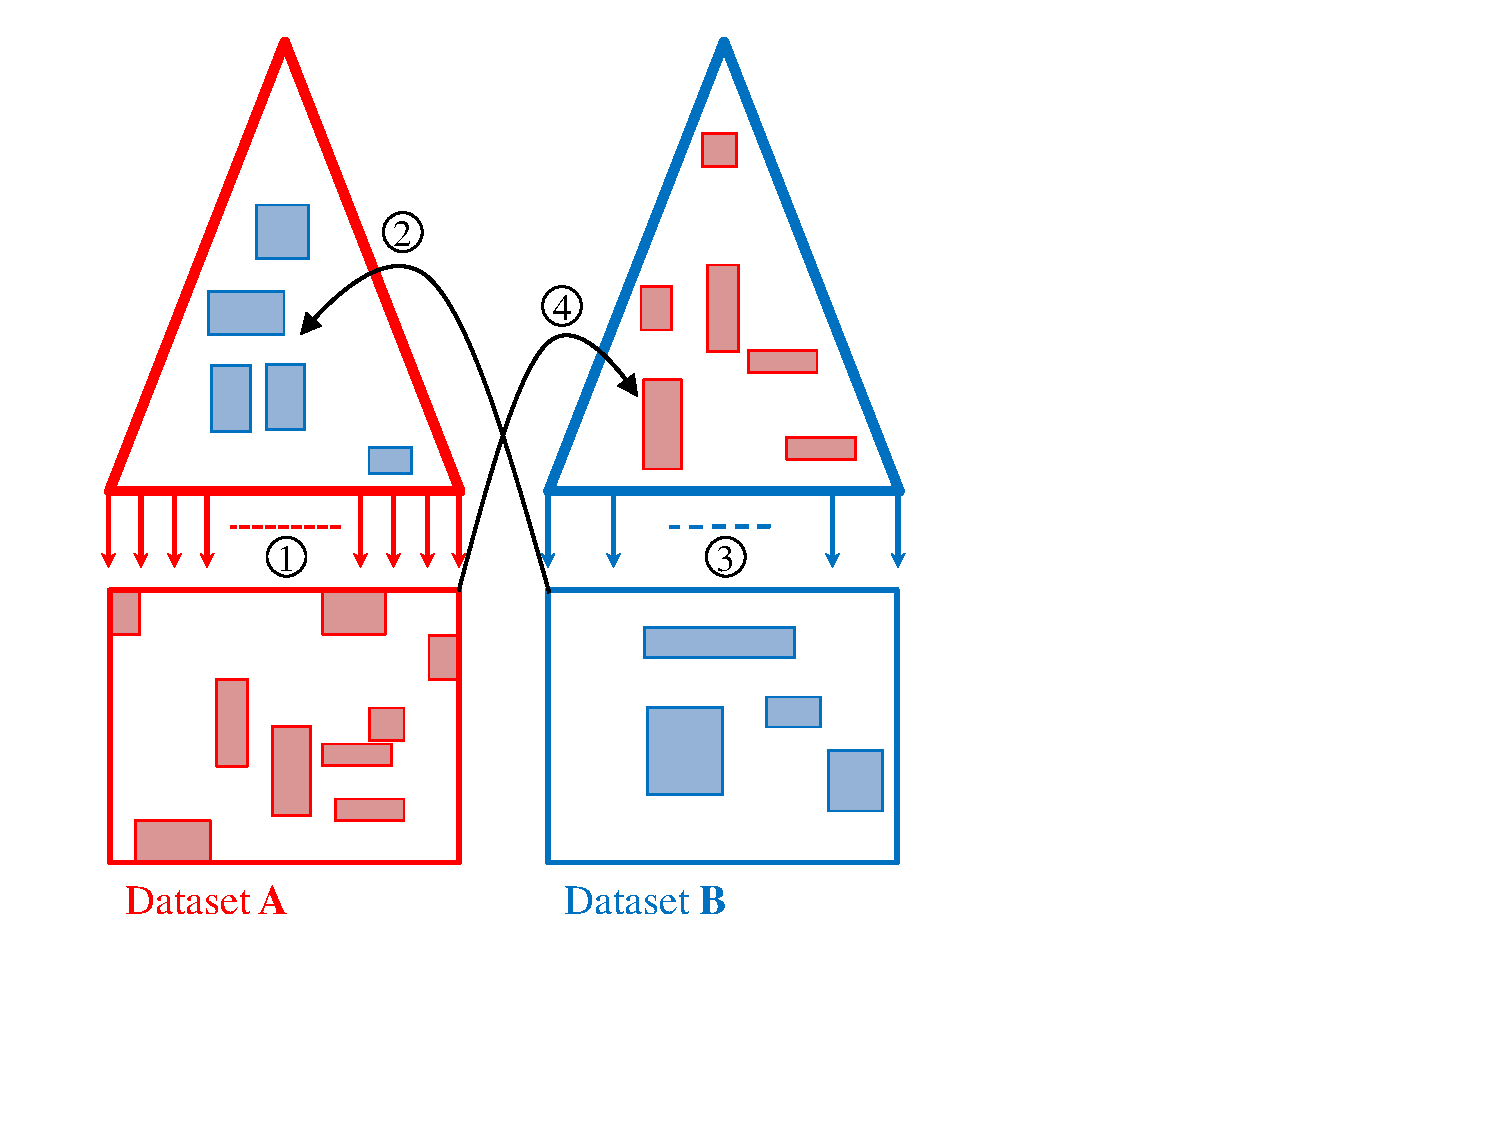
\includegraphics[width=.8\columnwidth]{figures/DTouch}
        \caption{{\dSJ} algorithm procedure}
        \label{fig:DTOUCH}
      \end{center}
\end{figure}

This modification is based on building two separate R-trees. First step is building R-tree using objects from dataset A, the same as in {\SJ}. Then, we assign objects of dataset B to this tree. During the assignment phase the level of the node where we decide to assign our object represents the workload for the joining step. Since every assigned object must be checked with all the objects in the descendant leafs nodes, the lower level assignment requires less number of comparisons for joining\footnote{The number of descendants grows exponentially with the level.}. In dTOUCH we restrict assignment to high levels of the tree. The restriction avoids assigning many objects of dataset B to higher levels of the tree built from objects of dataset A, $T_A$. And in return, for the objects of dataset B that has not been assigned to $T_A$, we have to create another tree, $T_B$, to compensate the missing results of the not assigned objects of the dataset B. The decision of whether assigning an object of B to level $l$ of the $T_A$ that has $L_{T_A}$ levels is based on the following probability, $P^{B}_{T_A}$:
\begin{equation*}
{P^{B}_{T_A}}=e^{-\alpha\times\frac{l}{L_{T_A}}}\times(1-\frac{l}{L_{T_A}})
\end{equation*}
$P^{B}_{T_A}$ is the probability of assigning an object of dataset B to the tree of dataset A, $T_A$. The equation consists of an exponent part and a coefficient to the exponent part. The former part of the equation creates a fast decreasing curve starting from one and the latter part creates an end (when we are at the root level) of zero (to avoid assignment to the root) for the curve.  

\begin{wrapfigure}{l}{0.5\columnwidth}
    \centering
    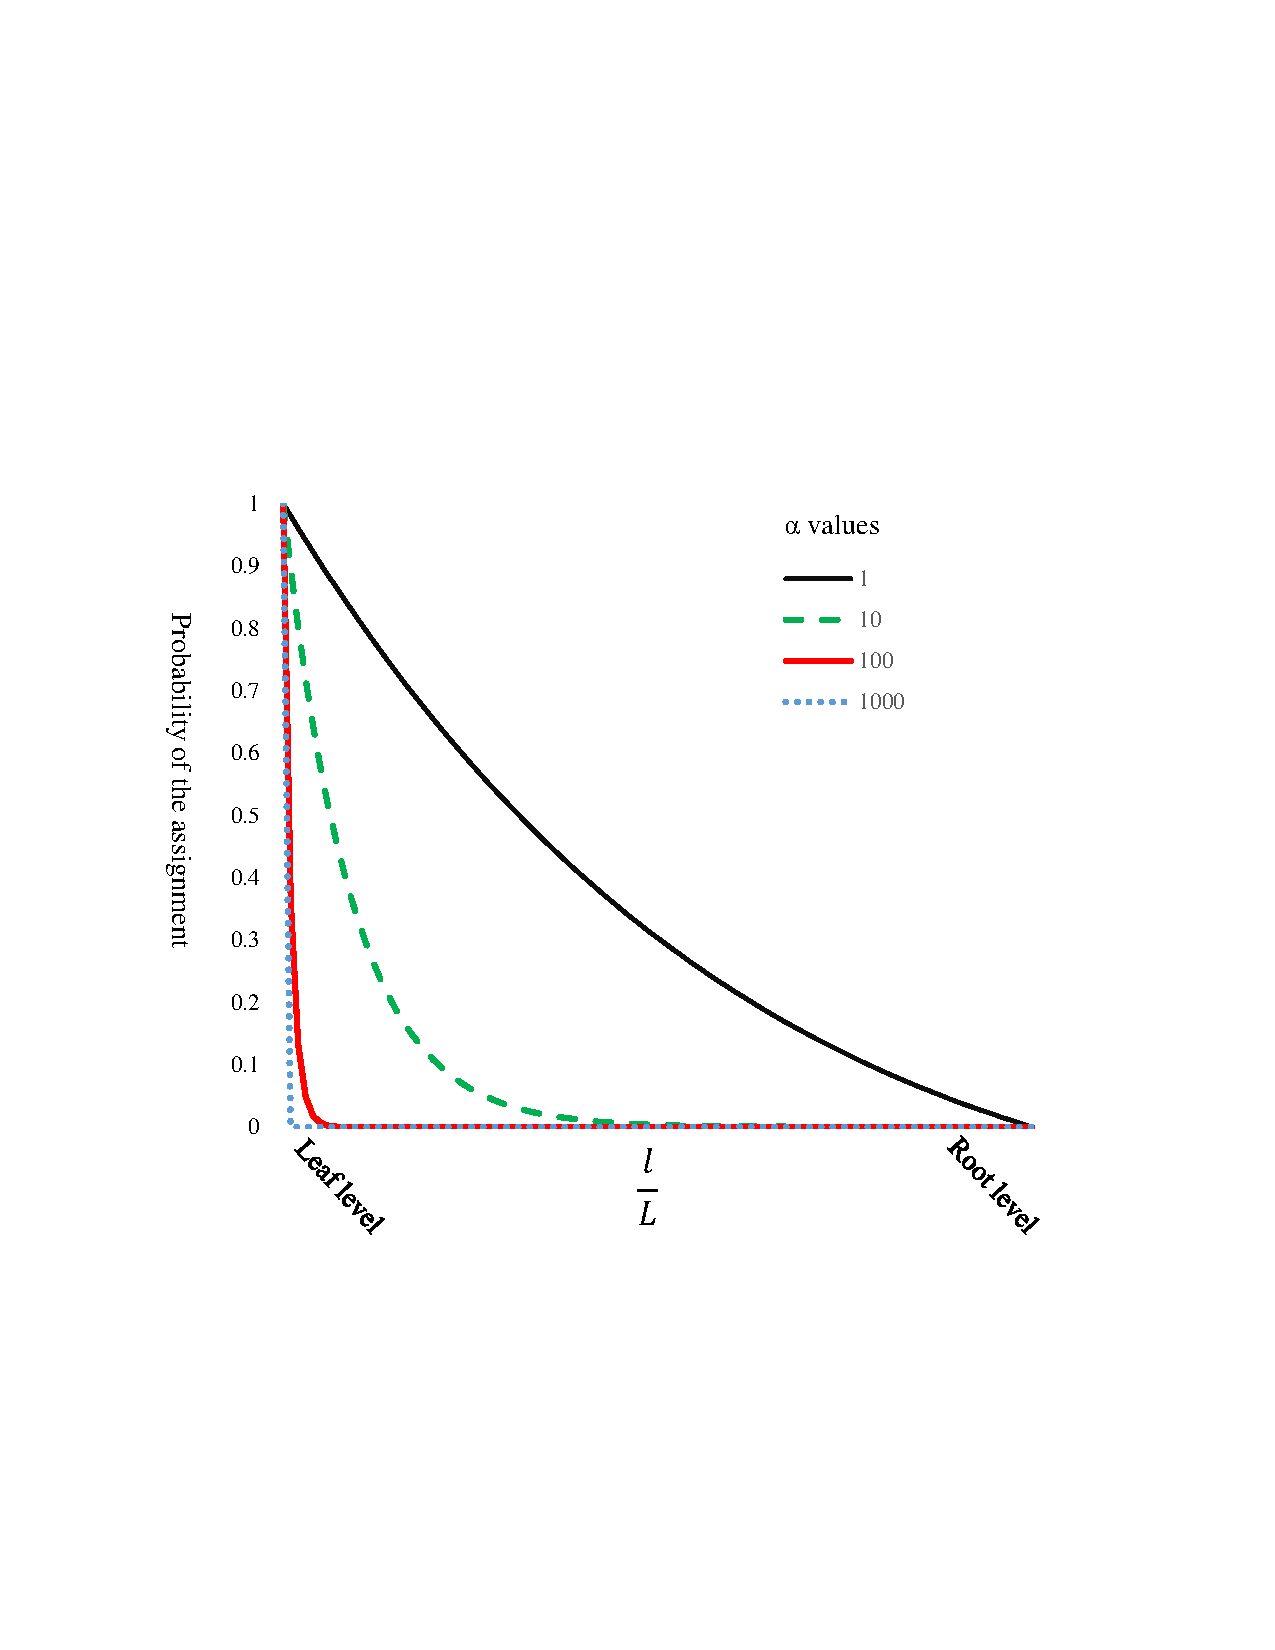
\includegraphics[width=0.48\columnwidth]{figures/alpha}
    \caption*{assignment coefficient $\alpha$.}
    \label{fig:alpha}
\end{wrapfigure}

This figure illustrates how different values of the coefficient $\alpha$ influences the assignment. In order to avoid many assignment to the root node ($\alpha=1$) on one hand and also let some objects to be assigned to high levels ($\alpha \geq 100$) on the other hand we choose $\alpha=10$.\\

After assigning objects of dataset B to $T_A$, {\dSJ} creates another R-Tree, $T_B$, for the remaining, not previously assigned, objects of dataset B. Then, {\dSJ} similarly assigns all the objects of dataset A to $T_B$. Finally, {\dSJ} joins each tree, $T_A$ and $T_B$, with their assigned objects similar to the algorithm \ref{alg:touchjoin}.

\begin{algorithm}
\caption{dTOUCH algorithm, Assignment restriction part}\label{alg:DTOUCH}
\begin{algorithmic}[1]
\Function{assignment}{$dataset_B$}
\setcounter{ALG@line}{\ref{alg:assign:assigns}}
	\If{$|S|>1$}\Comment{assign with the following condition}
        \State{$r=$ generate a uniform random number $\in [0,1]$}
        \State{$l=$ level of $currentNode$}
        \If{$r \le P^{B}_{T_A}$}
	    \State{assign $b$ to $currentNode$}
	    \State{delete $b$ from $dataset_B$}
	  	\EndIf
	  	\State{\Continue}
	\EndIf
\EndFunction
\end{algorithmic}
\end{algorithm}

Figure \ref{fig:DTOUCH} illustrates the steps of {\dSJ} algorithm: 1) constructing $T_A$; 2) Assigning the objects of dataset B to the internal nodes of $T_A$ following algorithm \ref{alg:DTOUCH}; 3) constructing R-Tree for the remaining objects $B'$ of dataset B, $T_{B'}$; 4) assigning the objects of dataset A to $T_{B'}$ following algorithm \ref{alg:touchassign}.

\subsection{{\cSJ} algorithm (complex {\SJ})}

In our second attempt to reduce the asymmetric exist in {\SJ} instead creating two separate trees we create a single tree by allowing the objects of both datasets to be assigned to internal nodes of the tree. Therefore, {\cSJ} algorithm constructs one symmetric R-tree, using both datasets simultaneously.

\begin{wrapfigure}{l}{0.5\columnwidth}
    \centering
    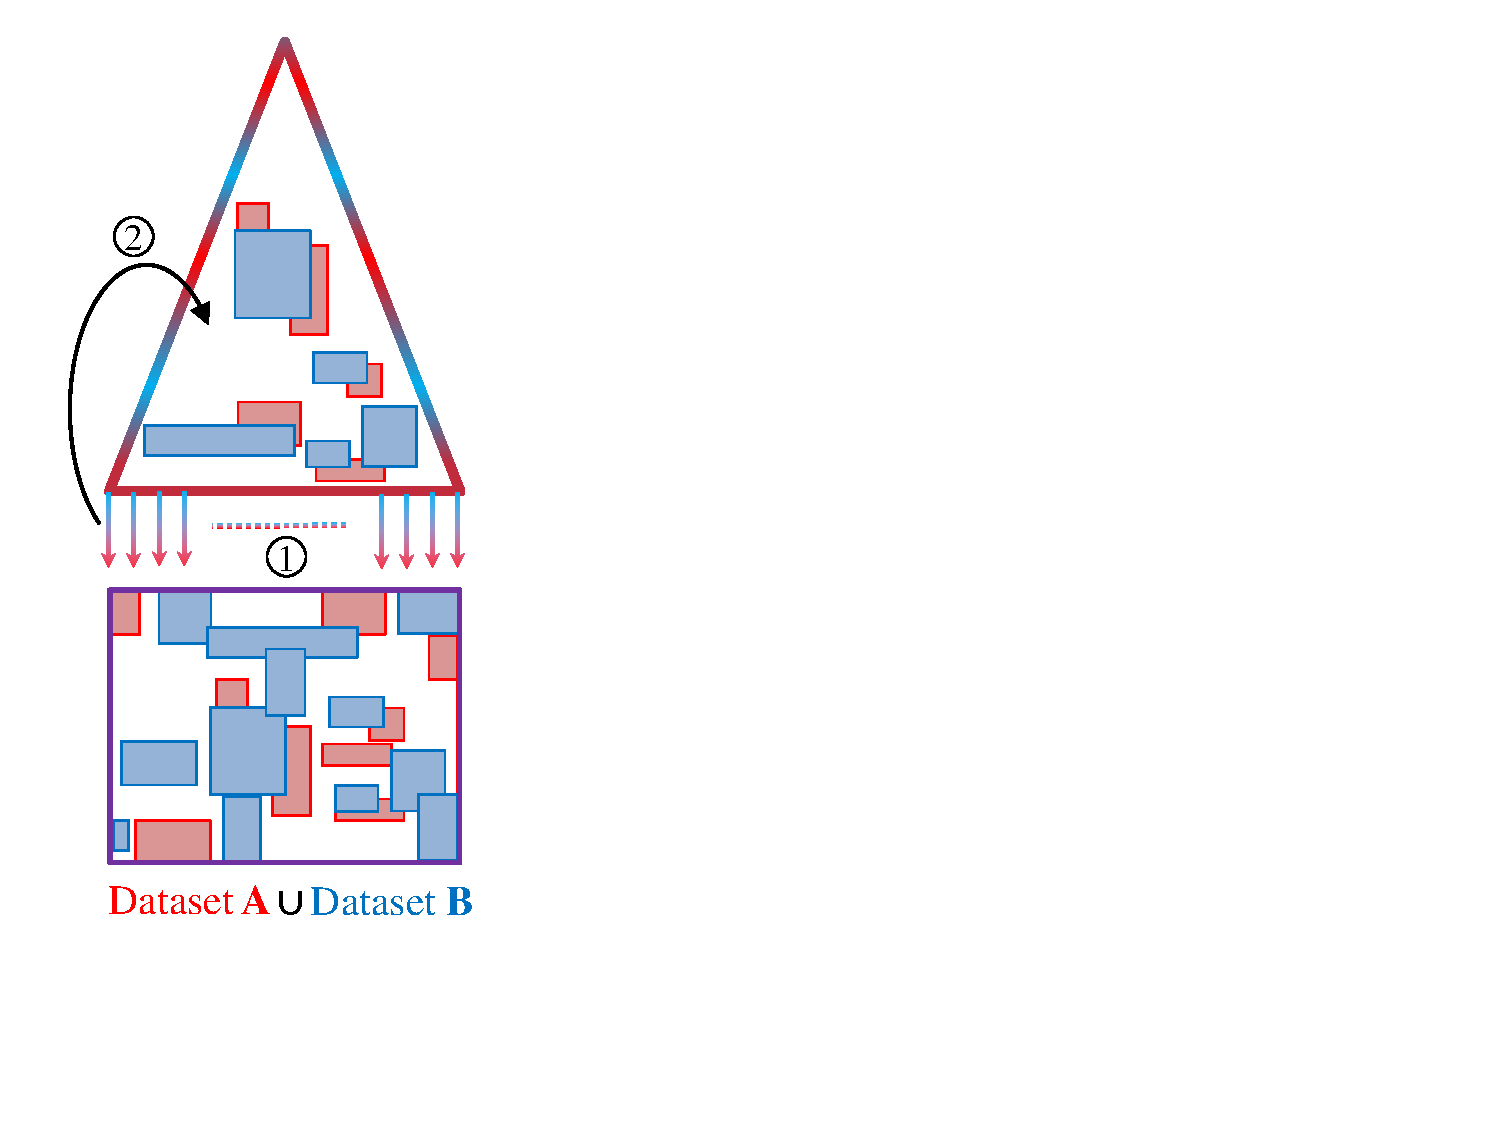
\includegraphics[width=0.48\columnwidth]{figures/CTouch}
%    \caption*{{\cSJ} algorithm procedure}
%    \label{fig:CTOUCH}
\end{wrapfigure}

To explain {\cSJ} we use colors in our definitions to distinguish datasets and MBRs types. We assume objects of dataset A and B be red $o^r$ and blue $o^b$ respectively. Following this coloring we will define six colors of MBRs. Given these assumptions we construct a single tree that contains both datasets’ objects assigned to any level of the tree by performing the tree construction (first step of {\SJ} algorithm) on a dataset that is a merge of both datasets A and B (Early merging).

This figure illustrates the steps of {\cSJ} algorithm: 1) constructing R-Tree for dataset $A \cup B$, $T_{A \cup B}$; 2) Moving the objects of the leaf level to the internal levels of $T_{A \cup B}$ following algorithm \ref{alg:CTOUCH}.

\subsection{Alvis {\cSJ}}
The key idea of rewriting TOUCH code is making the algorithm symmetric to A and B datasets. In this implementation we will try to build one symmetric R-tree, using both datasets as equally as possible. For pretty illustrating the principals of the approach lets introduce some colors and definitions. Let objects ($o$) from dataset A be red objects (\textcolor{red}{$o$}) and from dataset B - blue objects (\textcolor{blue}{$o$}). Each objects has its own MBR ($ \square $) that has corresponding color. Let MBR of the node $i$ on the level $l$ be red ($v^l_i \leftarrow \textcolor{red}{\square}^l_i$) if it was built as intersection of all red MBRs of the children ($\textcolor{red}{\square}^{l}_i = \bigcup\textcolor{red}{\square}^{l}_{i-1}$). Lets MBR of the node be blue if it was built from blue ones. Let MBR be black ($\square^{l}_i$) if it was build as intersection of blue and red MBRs. Let the assigned red objects be dark red ($\textcolor{red}{\blacksquare}^{l}_i$) and assigned blue - dark blue ($\textcolor{blue}{\blacksquare}^{l}_i$).

\subsubsection{Overview}Finished with colors, now the introduction to the algorithm goes. The algorithm consists of the same steps as original TOUCH: building, assignment and joining steps. During the building step we take all objects of both colors, build leaf nodes (create initial groups of objects) and build one mutual R-tree using Hilbert curve for indexing starting from leafs and creating two MBR per each node. Assignment phase is about taking all the objects from the leafs of the tree and assigning them to the tree traversing from the root to the leafs. At the joining step for each node we check the intersection of assigned object with all assigned objects which were assigned to the descenders of the node.

\paragraph{Reminder} $\square^{l}_i$ - MBR where $l$ - level in the tree, $i$ - index of the node where it must be located.

\subsubsection{Building phase}
See the algorithm \ref{alg:cTOUCHb}.

\begin{algorithm}
\caption{cTOUCH algorithm, Building phase}
\label{alg:cTOUCHb}
\begin{algorithmic}[1]
\State{$\textcolor{red}{\square}^{0}_i \leftarrow \textcolor{red}{o}_i$}
\State{$\textcolor{blue}{\square}^{0}_i \leftarrow \textcolor{blue}{o}_i$}
\State{$\forall j \quad v^0_j \leftarrow \textcolor{red}{\square}^{0}_i, \textcolor{blue}{\square}^{0}_i \quad i \in \{jC,jC+1,...,(j+1)C\}$}
\Comment{$C$ - leaf capacity}
\State{$\forall v^0_j \quad \square^{0}_j \leftarrow \textcolor{red}{\square}^{0}_j \cup \textcolor{blue}{\square}^{0}_j$}
\State{$\Omega \leftarrow v^0_j\quad \forall j$}

\While{size($\Omega$) $\neq 1$}
  \State{$v^{l}_i \leftarrow \Omega$}
  \State{Sort $v^l_i$ by $\square^{l}_i$ using Hilbert curve}
  \State{$\forall n \quad \omega_n \leftarrow v_i \quad i\in \{ jF, j(F+1), ..., (j+1)F\} $}
  \Comment{$F$ - fanout}
  \ForAll{$j$}
    \ForAll{$\textcolor{blue}{\square}^{l}_i, \textcolor{red}{\square}^{l}_i \leftarrow \omega_n$}
      \State{$\textcolor{blue}{\square}^{(l+1)}_j \leftarrow \bigcup_i \textcolor{blue}{\square}^{l}_i$}
      \State{$\textcolor{red}{\square}^{(l+1)}_j \leftarrow \bigcup_i \textcolor{red}{\square}^{l}_i$}
      \State{$v^{(l+1)}_j \leftarrow \textcolor{red}{\square}^{(l+1)}_j, \textcolor{blue}{\square}^{(l+1)}_j$}
      \State{$E \leftarrow (i,j)$}
      \Comment{$E$ - set of edges of the tree}
      \State{$\Omega \leftarrow v^{(l+1)}_j$}
    \EndFor
  \EndFor
\EndWhile
\State{Root $\leftarrow \Omega$}
\end{algorithmic}
\end{algorithm}


\subsubsection{Assignment phase}
See the algorithm \ref{alg:cTOUCHa}.

\begin{algorithm}
\caption{cTOUCH algorithm, Assignment phase}
\label{alg:cTOUCHa}
\begin{algorithmic}[1]
\ForAll{$v^0_i$}
  \ForAll{$\textcolor{red}{o} \leftarrow v^0_i$}
    \State{$v^l_j = $ Root}
    \Loop
      \State{$\omega = \{v^{l-1}_k : o^r \cap (\textcolor{blue}{\square}^{(l-1)}_k \cup \textcolor{blue}{\blacksquare}^{(l-1)}_k) \neq \varnothing , (k,j) \in E$ \} }
      \If{$\omega = \varnothing$}
	\State{Filter $\textcolor{red}{o}$}
	\State{Break}
      \EndIf
      \If{size($\omega$) $= 1$}
	\State{$v^l_j \leftarrow \omega$}
      \EndIf
      \If{size($\omega$) $> 1$ or $v^l_j$ - leafnode}
	\State{$v^l_j \leftarrow \textcolor{red}{o}$}
	\For{$l' \geq l$}
	  \State{$\textcolor{red}{\blacksquare}^{l'}_k \leftarrow \textcolor{red}{\square}^{l}_j \quad \forall (k,j) \in E$}
	\EndFor
	\State{Break}
      \EndIf
    \EndLoop
  \EndFor
  \State{Delete $\textcolor{red}{\square}^{0}_i$}
  \ForAll{$l > 0$ and $k : (k,i) \in E$}
    \State{$\textcolor{red}{\square}^{l}_k \leftarrow \bigcup_j\textcolor{red}{\square}^{(l-1)}_j \quad \forall j : (j,k) \in E$}
  \EndFor

  \ForAll{$\textcolor{blue}{o} \leftarrow v^0_i$}
    \State{$v^l_j = $ Root}
    \Loop
      \State{$\omega = \{v^{l-1}_k : \textcolor{red}{o} \cap (\textcolor{red}{\square}^{(l-1)}_k \cup \textcolor{red}{\blacksquare}^{(l-1)}_k) \neq \varnothing , (k,j) \in E$ \} }
      \If{$\omega = \varnothing$}
	\State{Filter $\textcolor{blue}{o}$}
	\State{Break}
      \EndIf
      \If{size($\omega$) $= 1$}
	\State{$v^l_j \leftarrow \omega$}
      \EndIf
      \If{size($\omega$) $> 1$ or $v^l_j$ - leafnode}
	\State{$v^l_j \leftarrow \textcolor{blue}{o}$}
	\For{$l' \geq l$}
	  \State{$\textcolor{blue}{\blacksquare}^{l'}_k \leftarrow \textcolor{blue}{\square}^{l}_j \quad \forall (k,j) \in E$}
	\EndFor
	\State{Break}
      \EndIf
    \EndLoop
  \EndFor

  \ForAll{$l > 0$ and $k : (k,i) \in E$}
    \State{$\textcolor{blue}{\square}^{l}_k \leftarrow \bigcup_j\textcolor{blue}{\square}^{(l-1)}_j \quad \forall j : (j,k) \in E$}
  \EndFor
\EndFor
\end{algorithmic}
\end{algorithm}

\subsubsection{Joining phase}

See the algorithm \ref{alg:cTOUCHj}.

\begin{algorithm}
\caption{cTOUCH algorithm, Joining phase}
\label{alg:cTOUCHj}
\begin{algorithmic}[1]
\ForAll{$v^l_i$}
  \ForAll{$\textcolor{red}{o} \leftarrow v^l_i$}
    \ForAll{$v^{l'}_j : l' \leq l, j \in E$}
      \ForAll{$\textcolor{blue}{o} \leftarrow v^{l'}_j$}
	\If{$\textcolor{blue}{o} \cap \textcolor{red}{o} \neq \varnothing$}
	  \State{Result $\leftarrow (\textcolor{red}{o}, \textcolor{blue}{o})$}
	\EndIf
      \EndFor
    \EndFor
  \EndFor

  \ForAll{$\textcolor{blue}{o} \leftarrow v^l_i$}
    \ForAll{$v^{l'}_j : l' \leq l, j \in E$}
      \ForAll{$\textcolor{red}{o} \leftarrow v^{l'}_j$}
	\If{$\textcolor{red}{o} \cap \textcolor{blue}{o} \neq \varnothing$}
	  \State{Result $\leftarrow (\textcolor{red}{o}, \textcolor{blue}{o})$}
	\EndIf
      \EndFor
    \EndFor
  \EndFor

  \ForAll{$\textcolor{blue}{o}, \textcolor{red}{o} \leftarrow v^l_i$}
      \If{$\textcolor{blue}{o} \cap \textcolor{red}{o} \neq \varnothing$}
	\State{Result $\leftarrow (\textcolor{red}{o}, \textcolor{blue}{o})$}
      \EndIf
  \EndFor
\EndFor
\end{algorithmic}
\end{algorithm}

\subsection{{\reSJ} algorithm (redoing {\SJ})}

\begin{figure}[htb]
    \begin{center}
        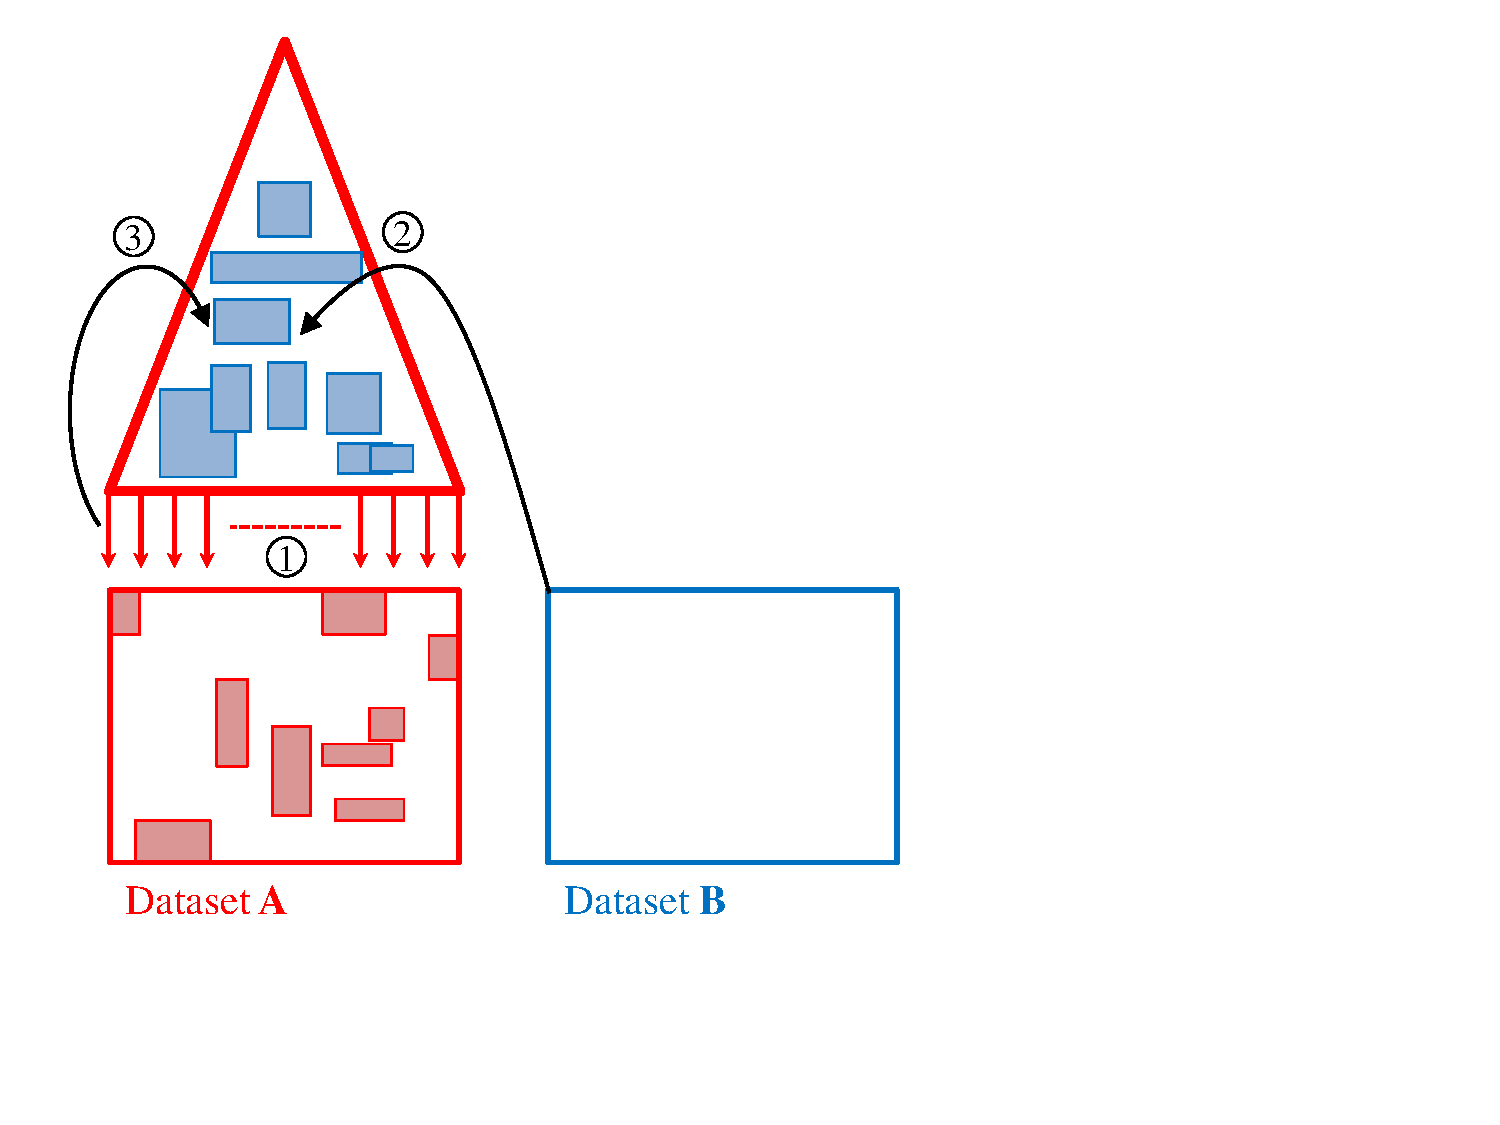
\includegraphics[width=.8\columnwidth]{figures/ReTouch}
        \caption{{\reSJ} algorithm procedure}
        \label{fig:RETOUCH}
      \end{center}
\end{figure}

{\reSJ} algorithm avoids the so-called early merging of {\cSJ} while creates a single tree for both datasets that contains their objects in any level. {\reSJ} algorithm first constructs a tree that is formed\footnote{without assigning them to the tree} by the objects of dataset A, then assigns the objects of dataset B to this tree without any level restriction. Given this tree that contains only objects of dataset B we reform the tree, then assign the objects of dataset A.

The last assignment, of dataset A, has a further filtering feature that we exploit.  While {\reSJ} assigns each object $a$ of A by traversing the $T_B$ starting from the root node. At each level, we move one level down iff $a$ overlaps with a single node's mbr. However, in the top-down traversal we may reach to a level that $a$ has no overlap with any node's mbr while $a$ had overlap with a node's self mbr before. Therefore, $a$ must be assigned to the lowest level that it overlaps with a node's self mbr of that level. Since $a$ has no overlap with any object below that level, we can assign $a$ in a way that avoids the redundant future comparisons of $a$ to the lower levels. Therefore, in {\reSJ} we distinguish these kind of assignments from the \emph{universal} assignments that we did for all the other algorithms.
As a result of this further filtering feature we introduce two types of assignment: \emph{universal} and \emph{top} assignment. The latter assignment indicates that there is no overlap with objects below, in contrast to the former assignment that has this below overlap.

Figure \ref{fig:RETOUCH} illustrates the steps of {\reSJ} algorithm: 1) constructing $T_{A}$; 2) assigning objects of dataset B to $T_A$ following algorithm \ref{alg:touchassign}; 3) Moving the objects of the leaf level to the internal levels of $T_{A}$ following algorithm \ref{alg:RETOUCH}.

\subsection{Balancing control}
In this subsection we explain how we enforce balancing by defining a cost function per object.

\hide{


\subsection{Cost of object}
In both cTOUCH and dTOUCH implementation each object has a cost $Z$. This number shows approximate upper bound for number of comparisons of this object with every object of opposite type in the descender nodes during the Join phase. Due to independence of the processing of each object during the joining phase, they can be distributed among processors and must be distributed equally in the meaning of workload. Having such cost number we can implement greedy algorithm to distribute tasks between processors. Cost is calculated using the information about the number of MBRs which intersects with the object. This number is calculated during the assignment phase (for all implementations of TOUCH) and it must be calculated anyway either we use cost estimation or not. So, we do not increase time for assignment step. Given the number of intersections with MBRs of children, $c$, lets estimate cost for cTOUCH and dTOUCH.
\paragraph{dTOUCH} Here objects are assigned in nodes but can be joined only with objects in leafs. So, given the level of our assigned object $l$, we have $cF^l$ leafs each containing $C$ objects. Here, we assume that on each level below our object intersect with every MBR of opposite type and there are $F$ (fanout) MBRs on each level.
$$ Z = cCF^l$$
\paragraph{cTOUCH}
Here objects can be joined at every node and every level of the tree. So, we will calculate the number of possible comparisons during the assignment step. Each time we assign an object to the node, we add 1 to every assigned object of the opposite type in every ancestor of the node.
$$Z(\textcolor{red}{o}_i \leftarrow v^l_i) = N\{o^b_j \leftarrow v^{l'}_j : (i,j) \in E \quad \& \quad l' > l\}$$


}

\section{Implementation}
\label{s_implementation}
In order to implement \SJ~we build in a first phase a tree based on dataset $A$. Each node in the tree contains a triple \{\emph{children}, \emph{MBR},
\emph{entities}\}. The leaf nodes contain as entities the objects of dataset $A$ and each node's MBR encloses all objects in it. The MBR of an inner node is
computed recursively based on the MBRs of its children.

In the second phase, the objects $b \in B$ are distributed and stored as the entities of the inner nodes of the tree. Following Algorithm \ref{alg:assignment},
each object $b$ is assigned to the node with the smallest MBR that still covers it.

\subsection{Partitioning}
In the first phase \SJ~partitions the objects of dataset $A$ into buckets and builds a tree, similar to an R-Tree~\cite{rtree}.

In \SJ~we use the Sort-Tile-Recursive approach~\cite{str} to group the objects. This technique first sorts the MBRs on the first dimension. Then STR divides the
dataset into $P^{1/D}$ slabs, where $P$ is the number of partitions and $D$ is the number of dimensions, according to their current order.
Finally, STR recursively processes the remaining slabs using the remaining $D-1$ dimensions. STR typically produces leaf nodes with the smallest
MBRs~\cite{str} (also on higher levels) and thus allows for more effective filtering.

\subsection{Design Parameters}
\label{s_parameters}
In the course of building the data structures, i.e., the tree, and ultimately joining the datasets several parameters can be set and tuned. In the following we
discuss what they are and how they can have an impact on the performance.
% of the join.
%and will later validate our findings with experiments.

\subsubsection{Tree Parameters}
The tree built on dataset $A$ in the first phase of the join resembles an R-Tree and hence has tunable parameters like the size of the leaf nodes and the
fanout, i.e., the number of children each node has (except the leaf nodes). The size of the inner nodes depends on the assignment of dataset $B$ and can hence
not be known a priori.

For the disk-based R-Tree, the fanout defines the node size and is chosen such that the nodes fit on an integer number of disk pages. Because \SJ~is developed
for memory, disk restrictions no longer apply and we can choose fanout and node size more freely. The choice of the fanout, however, has an impact on the
performance.

\begin{wrapfigure}{l}{0.5\columnwidth}
    \centering
    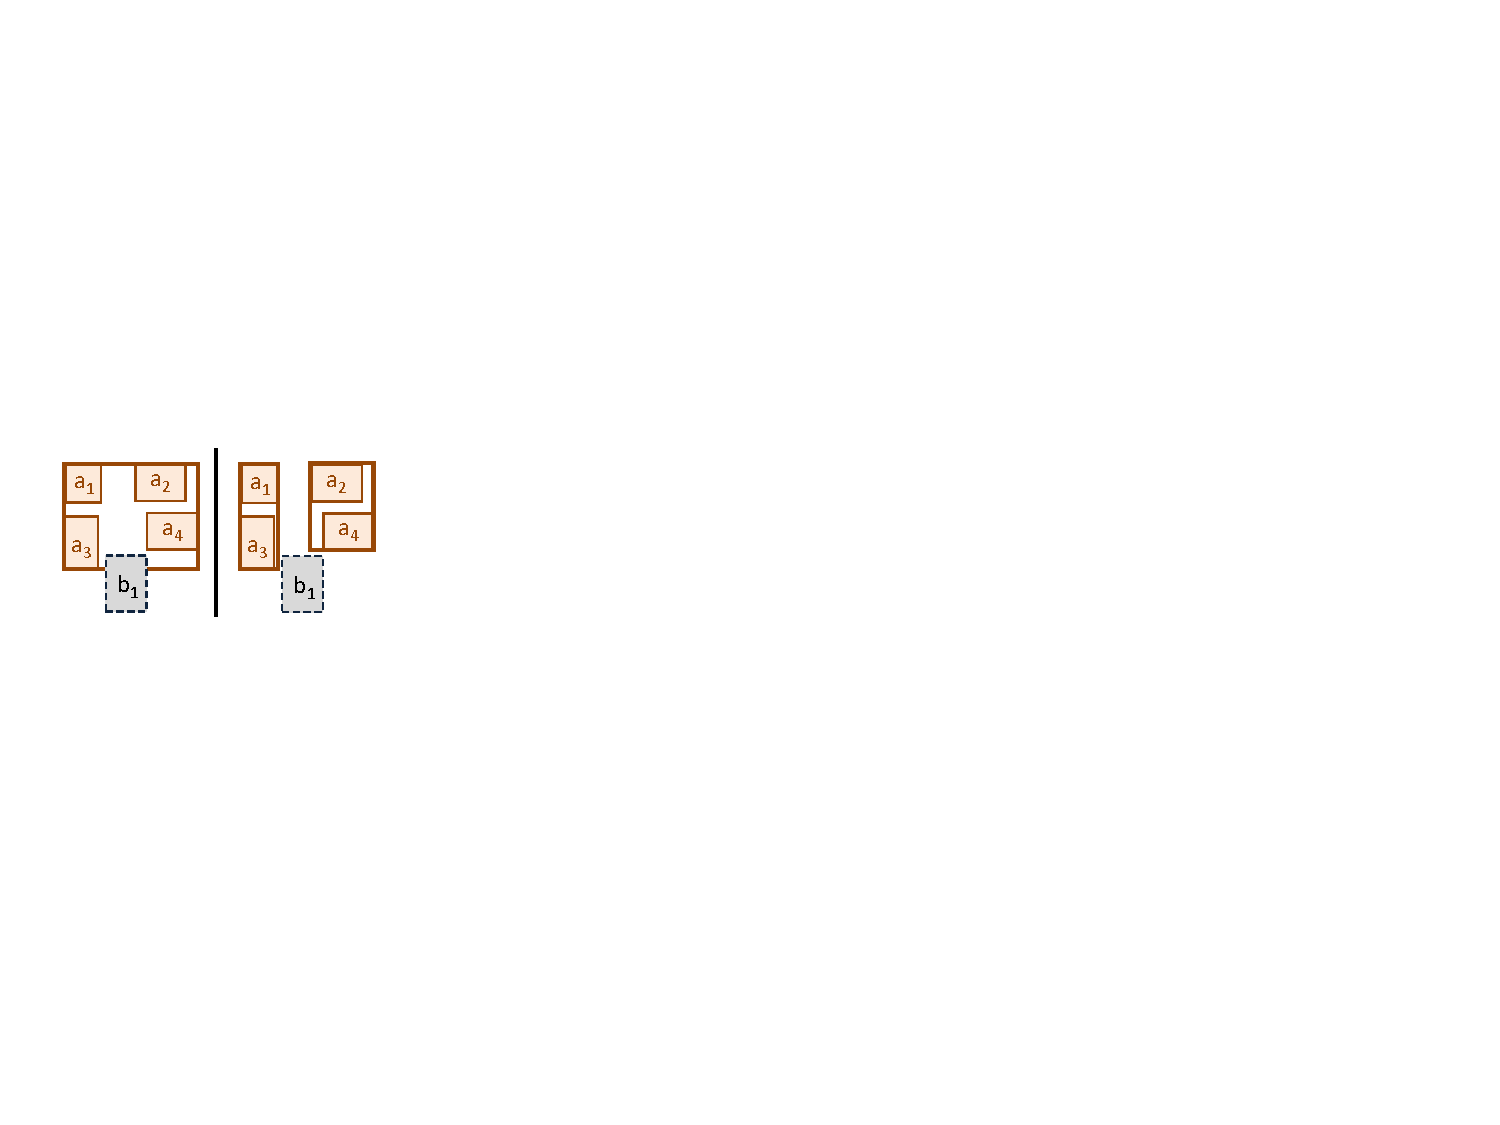
\includegraphics[width=0.48\columnwidth]{figures/filtering}
    \caption{Filtering.}
    \label{fig:filtering}
\end{wrapfigure}


\subsubsection{Local Join Parameters}
Local join is performed using Spatial Grid Hash (SGH) with dynamic resolution. Lets assume that SGH resolution is calculated for the node $V$ with assigned objects $a_1,a_2,...,a_m$. 
$$MBR(V) = \cup_{i=1..m} MBR(a_i)$$
$MBR(V)$ is the universe for SGH in $V$. The best resolution is one with each cell having equal size with an average assigned object, since in that case SGH does not have many duplications and it does not have many objects assigned to the single cell. For that reason we calculate the average size of assigned objects $a_1,...,a_m$ for each dimension and use that number for calculation of the resolution:
$$MBR_x(V) = \frac{1}{m}\sum_{i=1..m}MBR_x(a_i)$$
$$MBR_y(V) = \frac{\sum_{i=1..m}MBR_y(a_i)}{m}$$
$$MBR_z(V) = \frac{\sum_{i=1..m}MBR_z(a_i)}{m}$$


\subsubsection{Join Order}
\label{joinorder}
Given two datasets $A$ and $B$, deciding which dataset to use first to build the tree and which one to assign to the inner nodes of the tree is pivotal for
performance.

To improve filtering, the decision would ideally be based on the density of both datasets: the sparser the first dataset, the more objects of the second dataset
may be filtered. Not knowing the density of the datasets a priori, we can still make a reasonable assumption and take the smaller dataset as the first dataset.
If it has the same (or a bigger) spatial extent than the bigger dataset, then it will be sparser and allow for more filtering. If its spatial extent is smaller
than the one of the bigger dataset, then the difference in extent allows for effective filtering as well.

Using the smaller dataset first will also help to speed up building the hierarchical structure as well as reduce its size in memory.

\section{Experimental Evaluation}
\label{s_experimental_evaluation}

\subsection{Setup}
\label{s_setup}
% hardware setup

\subsection{Data description}
We used synthetic data for our experiments with different distributions of objects and. For each size of a dataset and for each distribution type we generated 10 samples. Three distributions are used: uniform , gauss and clustered (pic. \ref{fig:distributions}). Clustered distribution is objects that are randomly assigned to one of the cluster centers in the space and have a gauss distribution around the center of the cluster.
 
\begin{figure}{c}{}
    \centering
    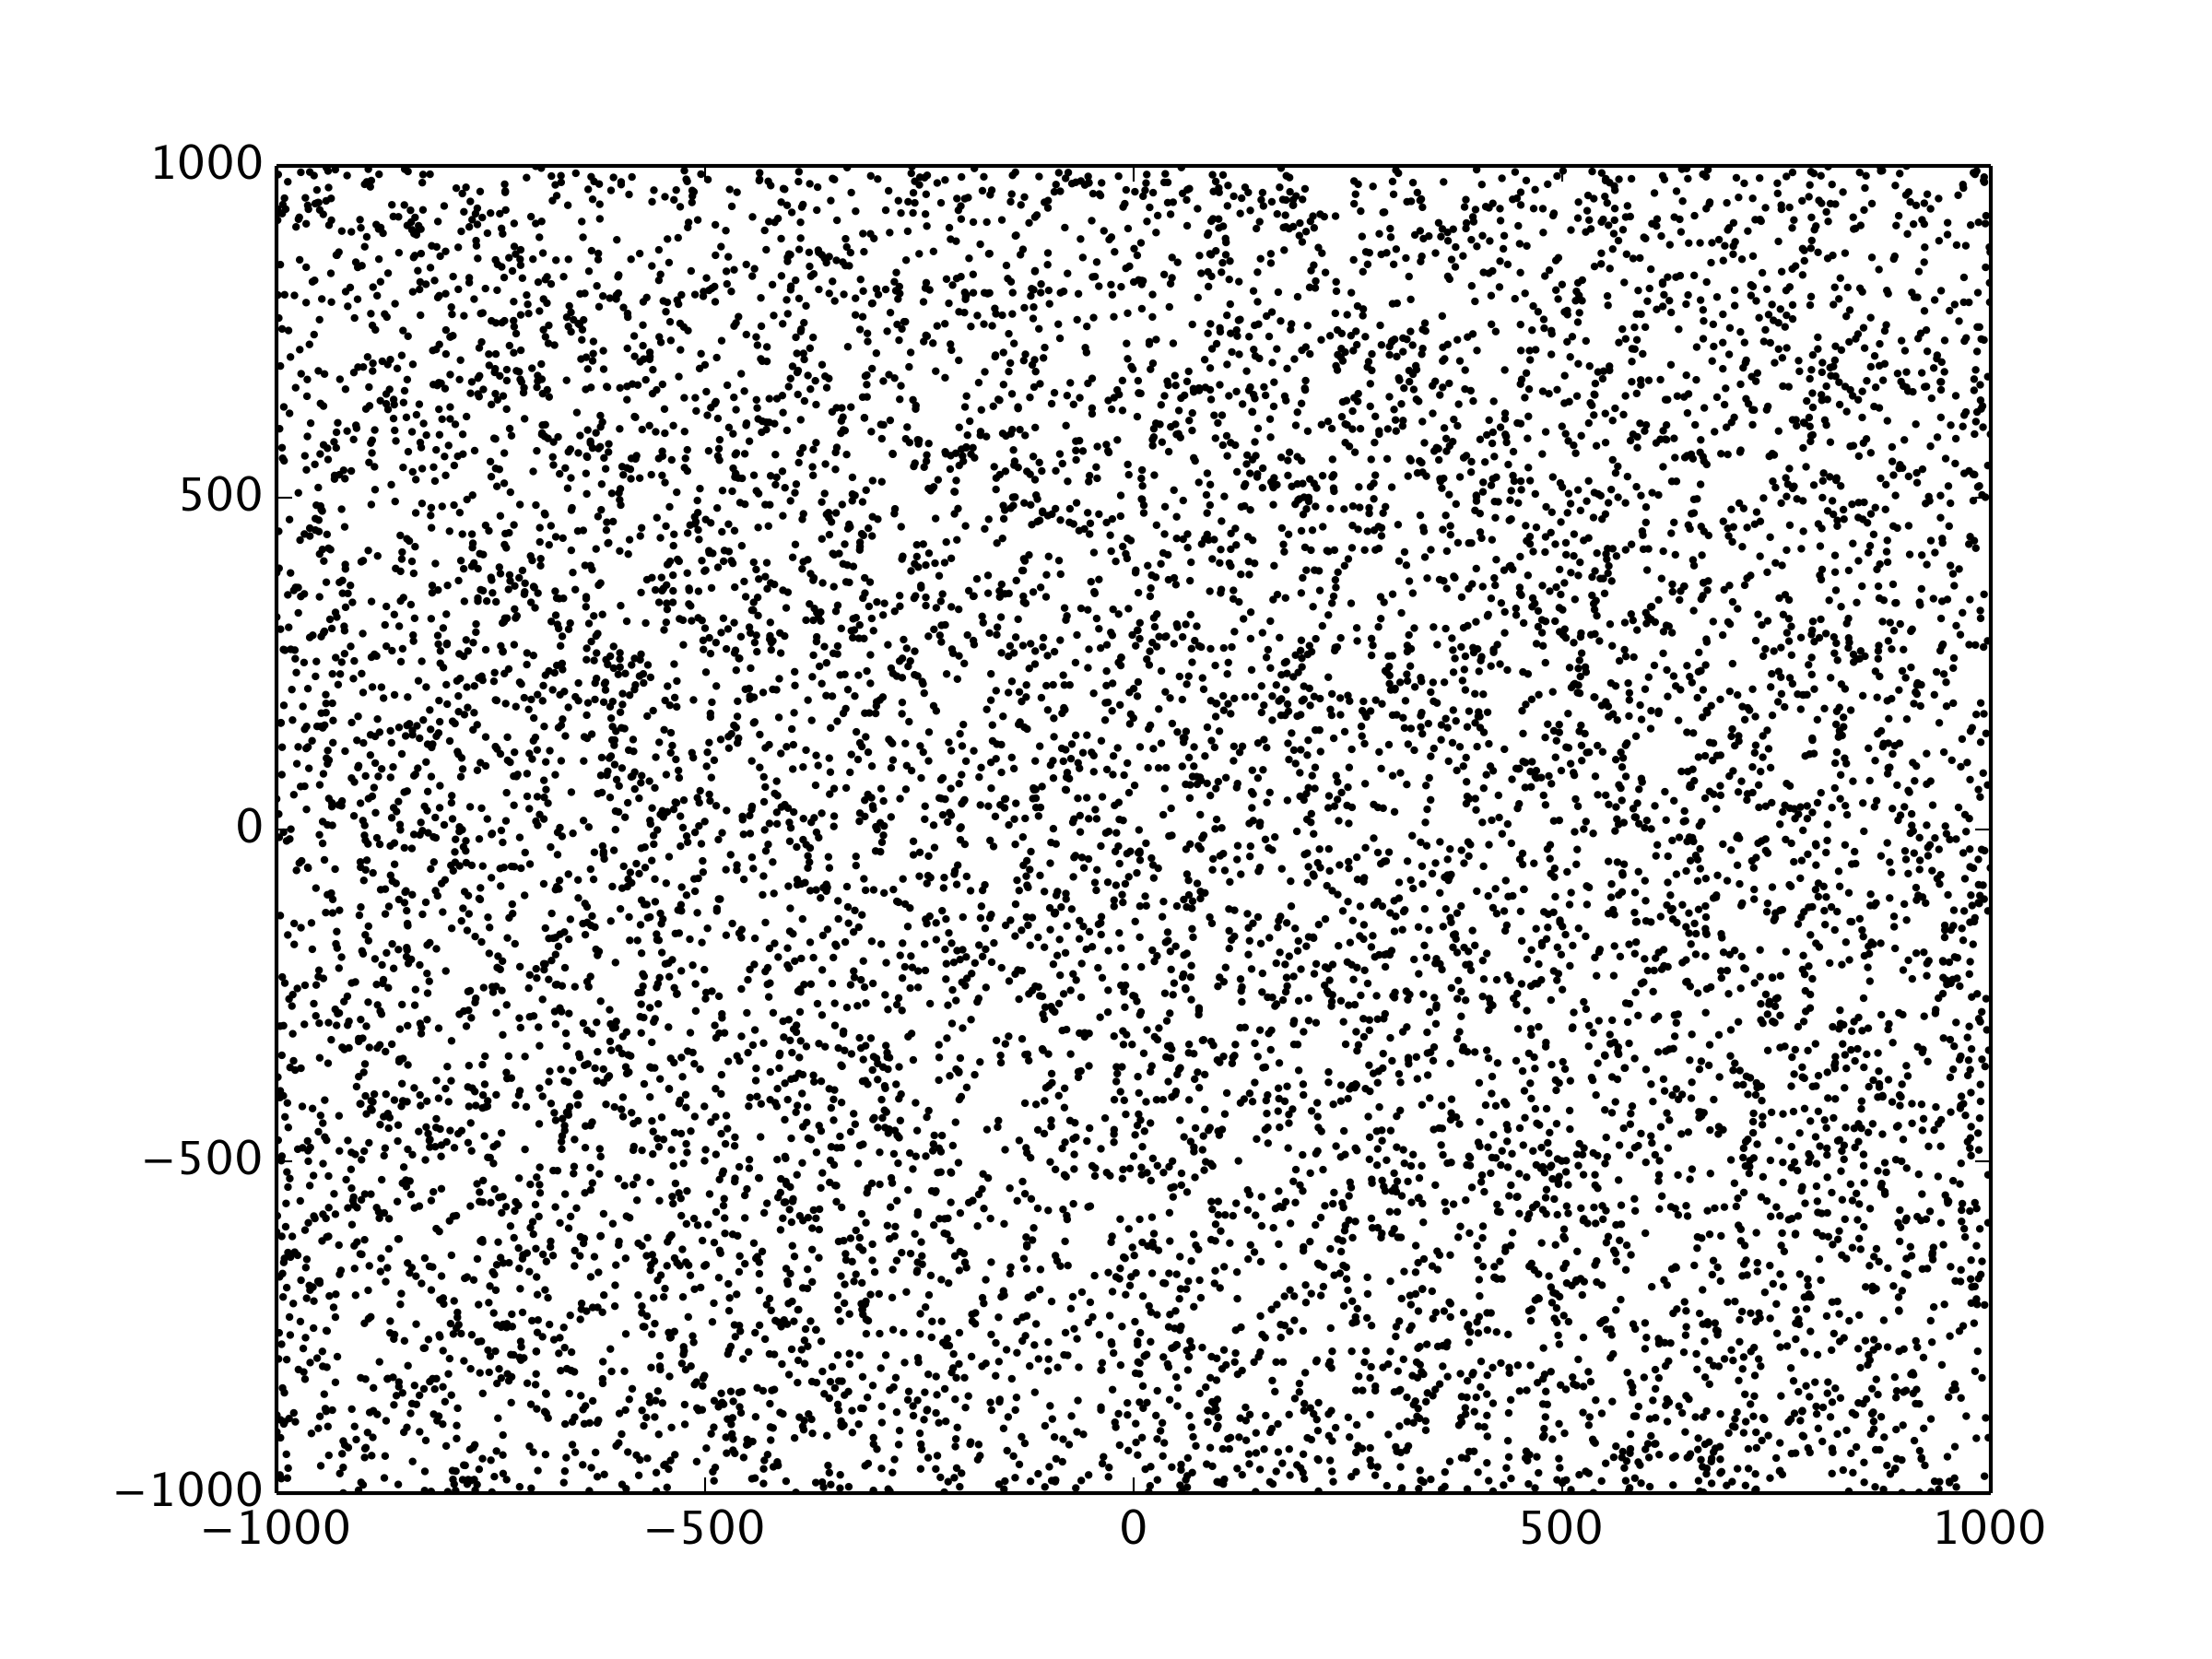
\includegraphics[width=0.3\columnwidth]{figures/picUni}
    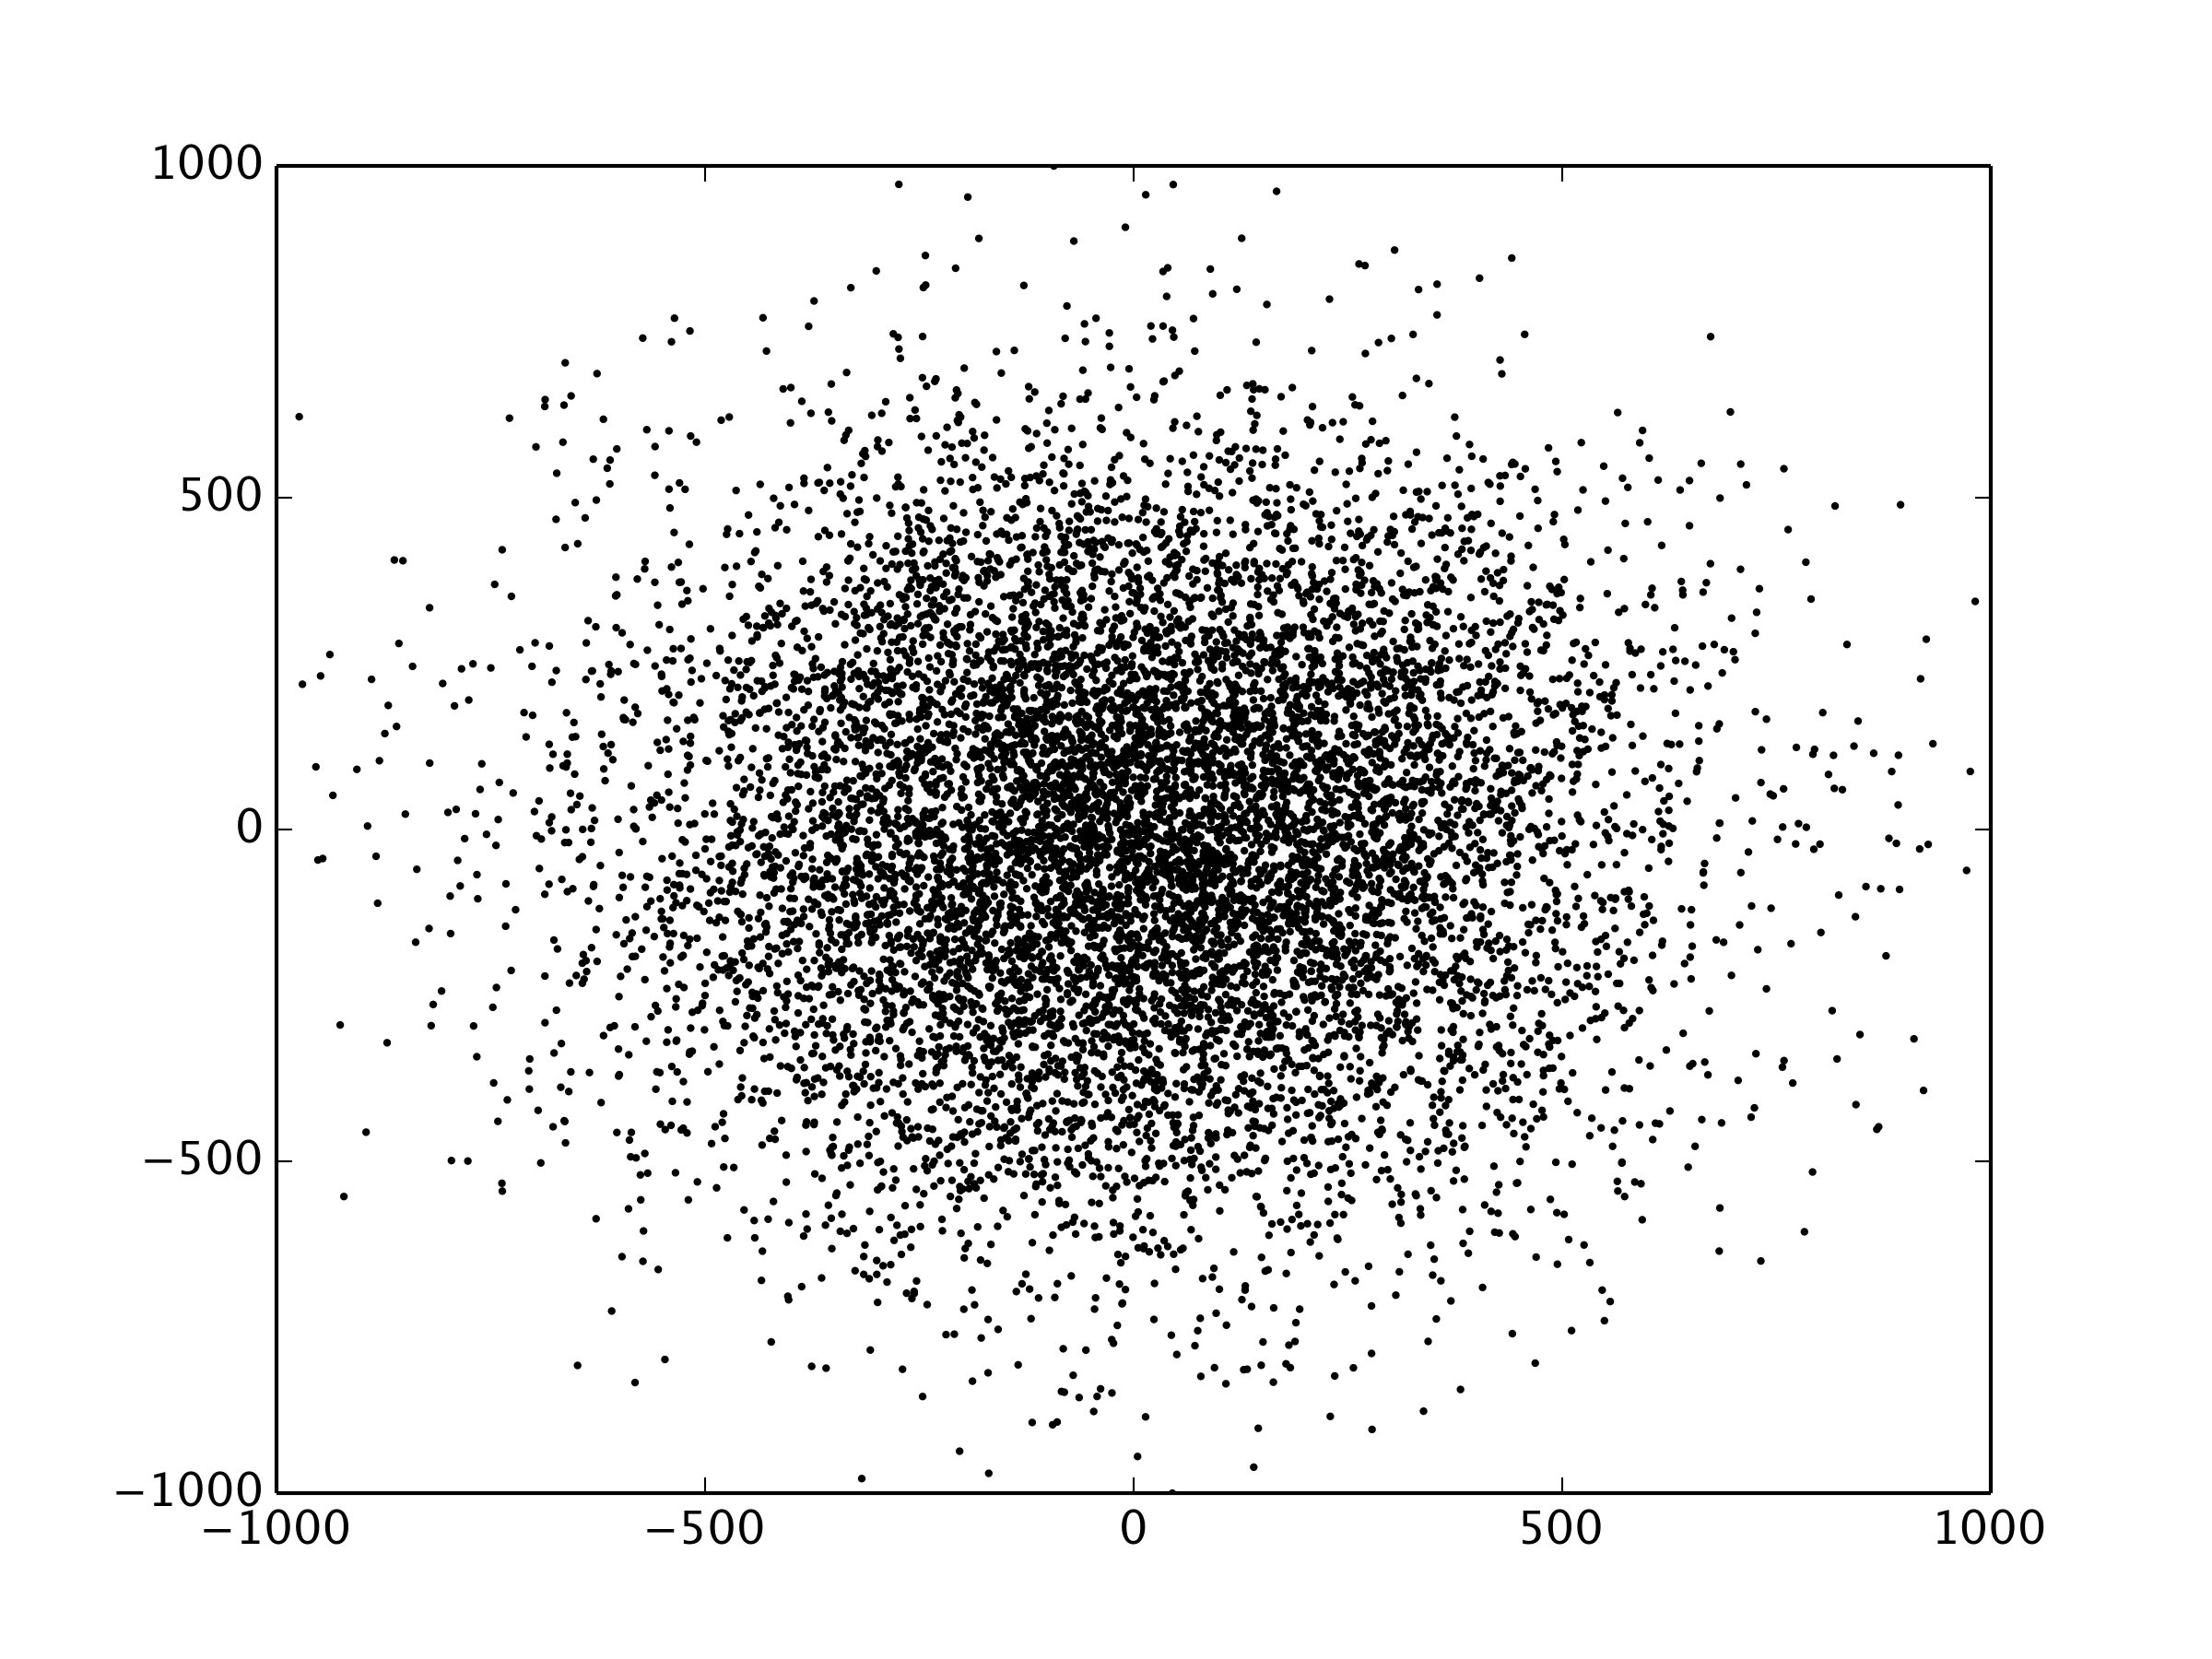
\includegraphics[width=0.3\columnwidth]{figures/picGauss}
    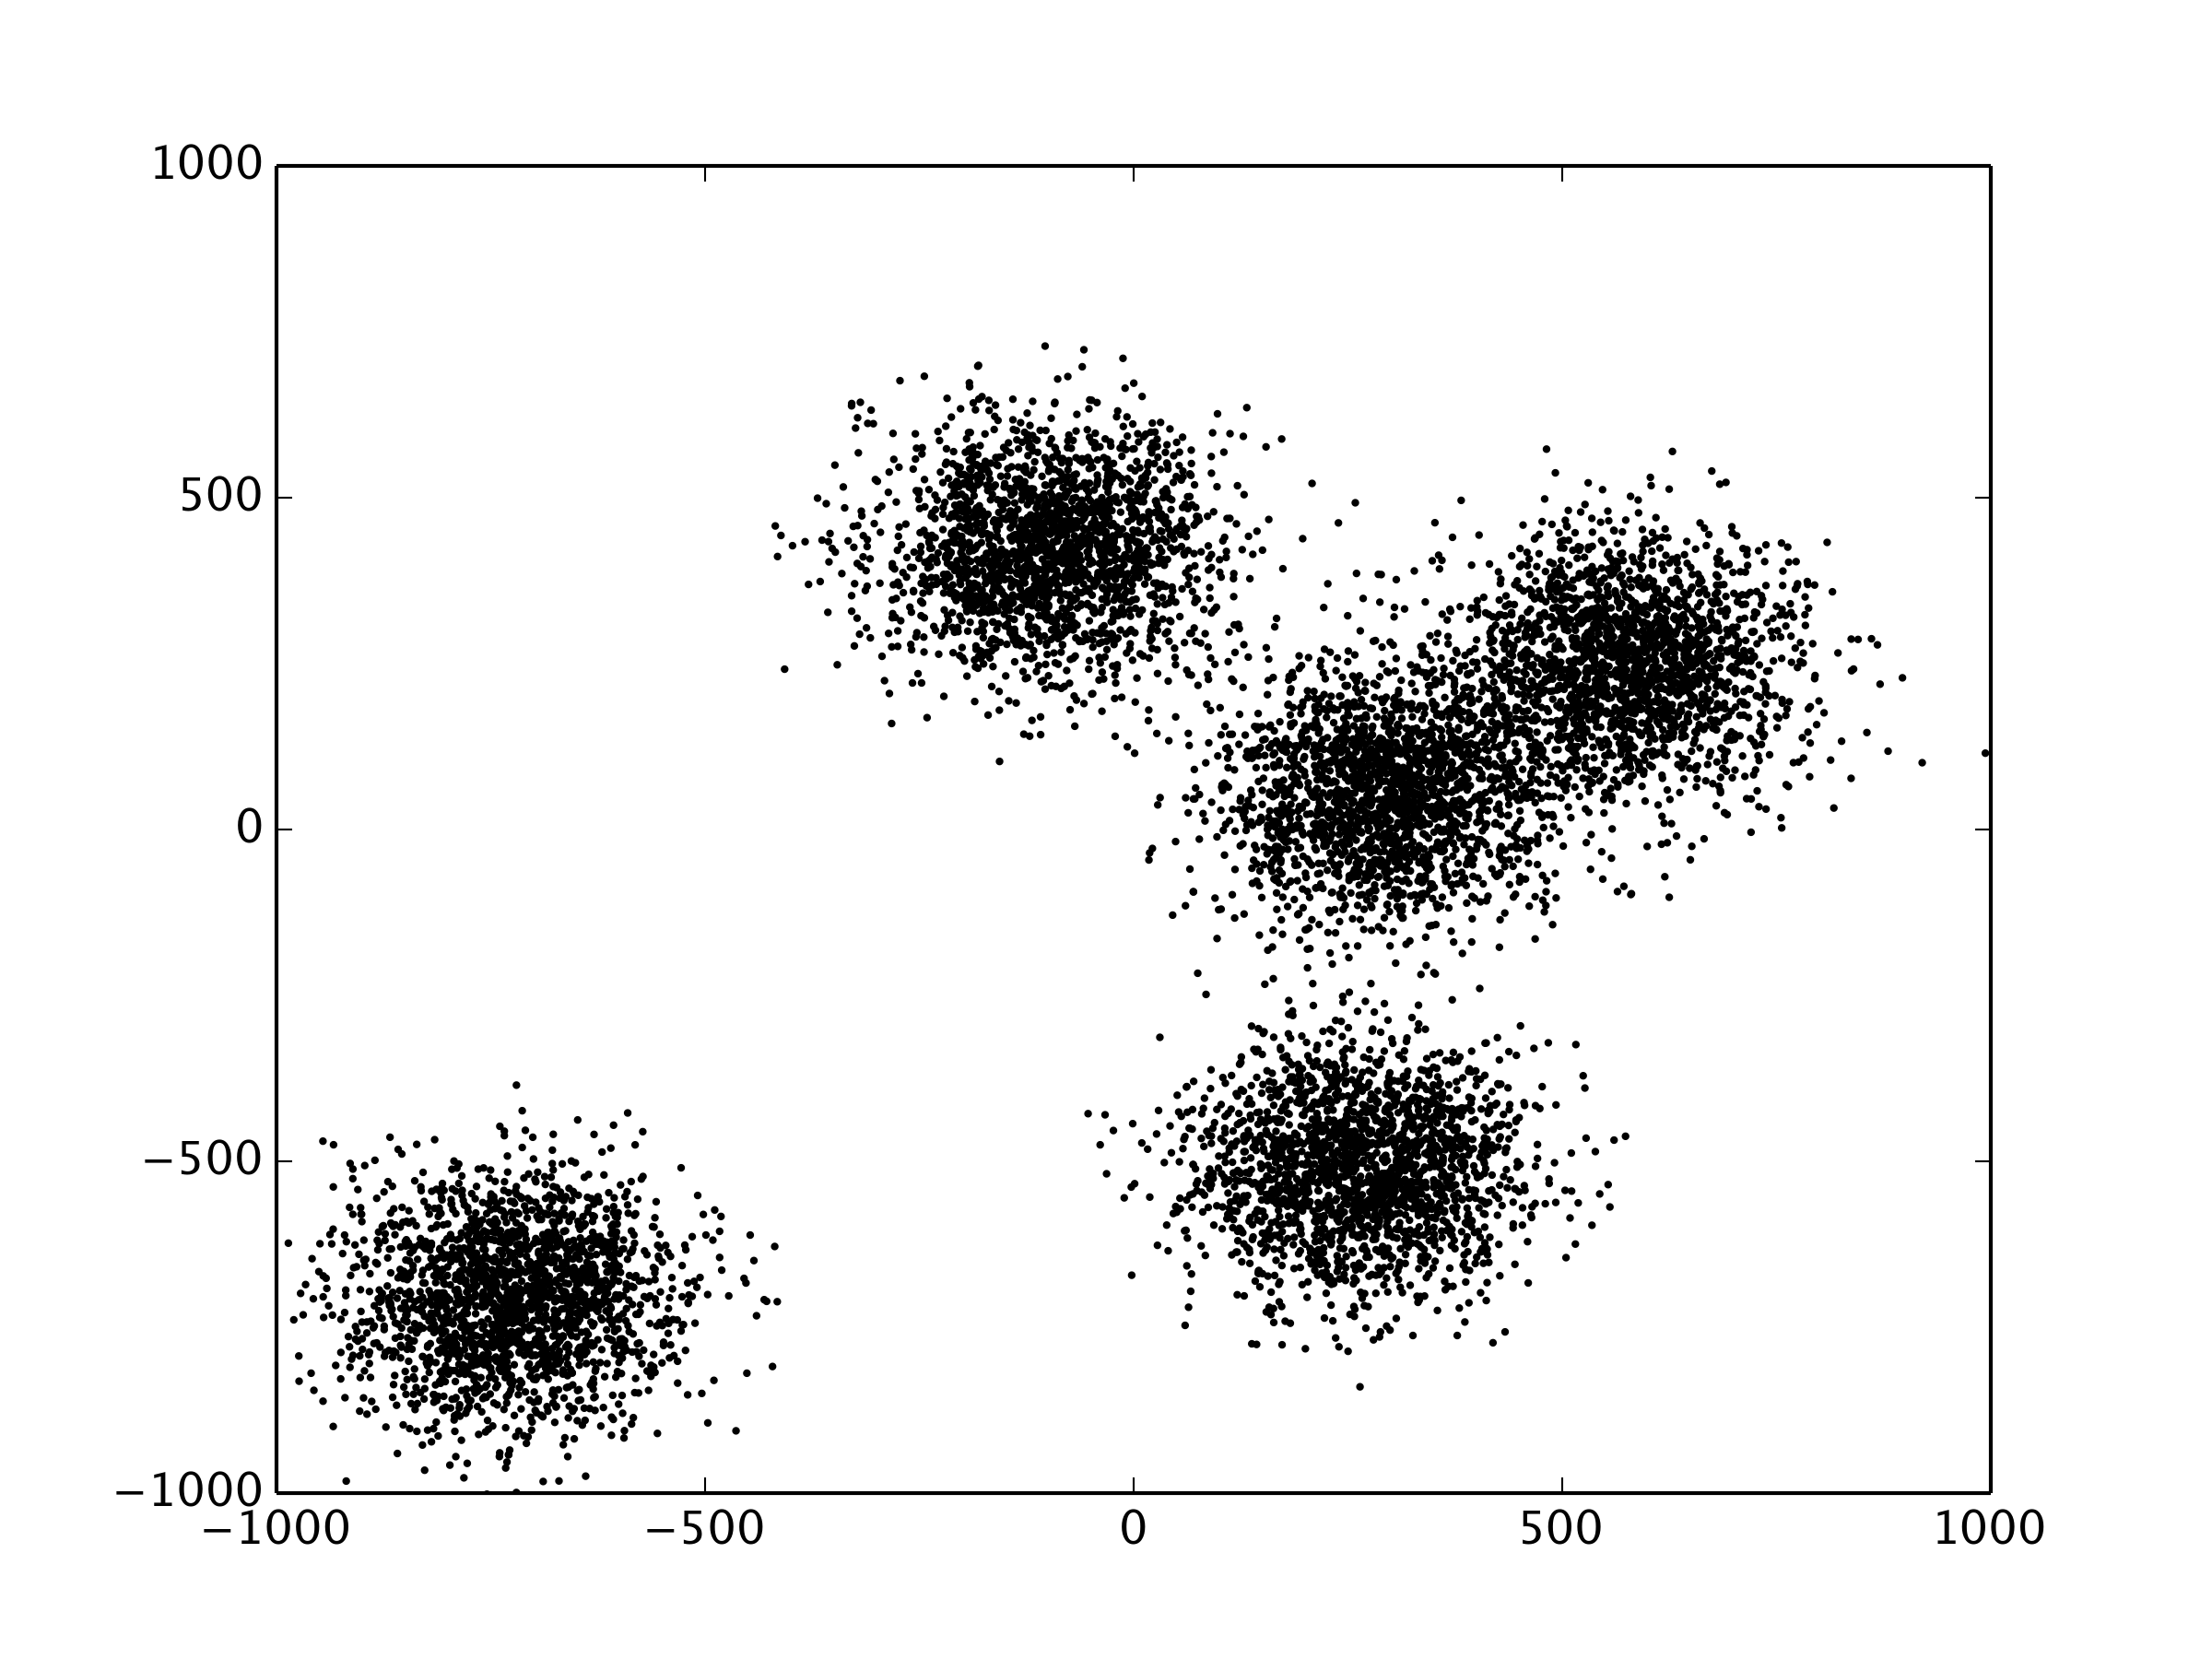
\includegraphics[width=0.3\columnwidth]{figures/picClust}
    \caption{Types of distributions of objects}
    \label{fig:distributions}
\end{figure}

\subsection{Experimental Methodology}
\label{experimentalmethodology}

\section{Conclusions}
\label{s_conclusions}
In this paper we identify the lack of efficient approaches for in-memory spatial joins. We demonstrate that the two in-memory approaches, namely the nested-loop
and the plane-sweep, are inefficient and that disk-based approaches are not efficient either when applied in main memory. An exception is PBSM, which is fast
but needs excessive memory.

We develop TOUCH, a spatial join algorithm that combines the advantages while avoiding the pitfalls of previous approaches. TOUCH avoids a space-oriented
partitioning on the large scale and uses a data-oriented partitioning to organize both datasets. To avoid object replication, objects of one dataset are used
to construct an R-Tree-like hierarchy, while those of the other are assigned to the level where they are fully contained by an MBR. The partitions on
different levels are joined using a space-oriented partitioning.

We experimentally demonstrate that our approach is faster and has a substantially smaller memory footprint than the previous state of the art with real and
synthetic datasets. Our results also indicate that TOUCH is scalable to larger and denser datasets, a key issue in scaling up the neuroscience application we
are motivated from. Thus, TOUCH is recommendable as a method of choice for such applications. Furthermore, as we only make a few assumptions about dataset
characteristics, with TOUCH we provide a general-purpose solution applicable on any spatial dataset.

\balance


\bibliographystyle{abbrv}
%\bibliography{sigfp132-nobari}
%\bibliographystyle{abbrvnat}

\begin{thebibliography}{10}
\vspace{2mm}

\bibitem{joinSelectivity}
W.~G. Aref and H.~Samet.
\newblock {A Cost Model for Query Optimization Using R-Trees}.
\newblock In {\em GIS '94}.

\bibitem{cascadedquadtree}
W.~G. Aref and H.~Samet.
\newblock {Cascaded Spatial Join Algorithms with Spatially Sorted Output}.
\newblock In {\em GIS '96}.

\bibitem{hashing}
W.~G. Aref and H.~Samet.
\newblock {Hashing by Proximity to Process Duplicates in Spatial Databases}.
\newblock In {\em CIKM '94}.

\bibitem{prtree}
L.~Arge, M.~de~Berg, H.~J. Haverkort, and K.~Yi.
\newblock {The Priority R-tree: a practically efficient and worst-case optimal
  R-tree}.
\newblock In {\em {SIGMOD '04}}.

\bibitem{sssj}
L.~Arge, O.~Procopiuc, S.~Ramaswamy, T.~Suel, and J.~S. Vitter.
\newblock {Scalable Sweeping-Based Spatial Join}.
\newblock In {\em VLDB '98}.

\bibitem{rstartree}
N.~Beckmann, H.-P. Kriegel, R.~Schneider, and B.~Seeger.
\newblock {The R*-Tree: an efficient and robust access method for points and
  rectangles}.
\newblock {\em SIGMOD Record}, 19(2):322--331, 1990.

\bibitem{join:RTree}
T.~Brinkhoff, H.-P. Kriegel, and B.~Seeger.
\newblock {Efficient Processing of Spatial Joins Using R-Trees}.
\newblock In {\em SIGMOD '93}.

\bibitem{deduplication}
J.-P. Dittrich and B.~Seeger.
\newblock {Data Redundancy and Duplicate Detection in Spatial Join Processing}.
\newblock In {\em ICDE 2000}.

\bibitem{databasefundamentals}
R.~Elmasri and S.~B. Navathe.
\newblock {\em Fundamentals of Database Systems}.
\newblock Addison Wesley, 3rd edition, 2000.

\bibitem{pais}
A.~Farris, A.~Sharma, C.~Niedermayr, D.~Brat, D.~Foran, F.~Wang, J.~Saltz,
  J.~Kong, L.~Cooper, T.~Oh, T.~Kurc, T.~Pan, and W.~Chen.
\newblock {A Data Model and Database for High-resolution Pathology Analytical
  Image Informatics}.
\newblock {\em Journal of Pathology Informatics}, 2(1):32, 2011.

\bibitem{tgstree}
Y.~J. Garc\'ia, M.~A. L\'opez, and S.~T. Leutenegger.
\newblock {A Greedy Algorithm for Bulk Loading R-trees}.
\newblock In {\em GIS '96}.

\bibitem{peptidefolding}
S.~Gnanakaran, H.~Nymeyer, J.~Portman, K.~Y. Sanbonmatsu, and A.~E. Garcia.
\newblock Peptide folding simulations.
\newblock {\em Current Opinion in Structural Biology}, 13(2):168--174, 2003.

\bibitem{rtree}
A.~Guttman.
\newblock {R-trees: a Dynamic Index Structure for Spatial Searching}.
\newblock In {\em SIGMOD '84}.

\bibitem{patchclamp}
O.~P. Hamill, A.~Marty, E.~Neher, B.~Sakmann, and F.~J. Sigworth.
\newblock {Improved Patch-clamp Techniques for High-resolution Current
  Recording from Cells and Cell-free Membrane Patches}.
\newblock {\em Pfl\"ugers Archiv European Journal of Physiology}, 391:85--100,
  1981.

\bibitem{spatialjointechniques}
E.~H. Jacox and H.~Samet.
\newblock {Spatial Join Techniques}.
\newblock {\em ACM TODS '07}.

\bibitem{index:HilbertRTree}
I.~Kamel and C.~Faloutsos.
\newblock {Hilbert R-tree: An Improved R-tree using Fractals}.
\newblock In {\em VLDB '94}.

\bibitem{join:SizeSeparation}
N.~Koudas and K.~C. Sevcik.
\newblock {Size Separation Spatial Join}.
\newblock In {\em SIGMOD '97}.

\bibitem{tabulating}
J.~Kozloski, K.~Sfyrakis, S.~Hill, F.~Sch\"urmann, C.~Peck, and H.~Markram.
\newblock {Identifying, Tabulating, and Analyzing Contacts Between Branched
  Neuron Morphologies}.
\newblock {\em {IBM} {J}ournal of {R}esearch and {D}evelopment},
  52(1/2):43--55, 2008.

\bibitem{str}
S.~Leutenegger, M.~Lopez, and J.~Edgington.
\newblock {STR: a Simple and Efficient Algorithm for R-Tree Packing}.
\newblock In {\em ICDE '97}.

\bibitem{join:Hash}
M.-L. Lo and C.~V. Ravishankar.
\newblock {Spatial Hash-Joins}.
\newblock In {\em SIGMOD '96}.

\bibitem{join:SeededTree}
M.-L. Lo and C.~V. Ravishankar.
\newblock {Spatial Joins Using Seeded Trees}.
\newblock In {\em SIGMOD '94}.

\bibitem{join:nonblocking}
G.~Luo, J.~F. Naughton, and C.~J. Ellmann.
\newblock A non-blocking parallel spatial join algorithm.
\newblock In {\em ICDE}, pages 697--705, 2002.

\bibitem{join:SlotIndex}
N.~Mamoulis and D.~Papadias.
\newblock {Slot Index Spatial Join}.
\newblock {\em IEEE TKDE}, 15(1):211--231, 2003.

\bibitem{joinprocessing}
P.~Mishra and M.~H. Eich.
\newblock {Join Processing in Relational Databases}.
\newblock {\em ACM Computing Surveys}, 24(1):63--113, 1992.

\bibitem{nobariGPU}
S.~Nobari, T.-T. Cao, P.~Karras, and S.~Bressan.
\newblock Scalable parallel minimum spanning forest computation.
\newblock In {\em Proceedings of the 17th ACM SIGPLAN symposium on Principles
  and Practice of Parallel Programming}, PPoPP '12, pages 205--214, New York,
  NY, USA, 2012. ACM.

\bibitem{twophasejoin}
J.~Orenstein.
\newblock {A Comparison of Spatial Query Processing Techniques for Native and
  Parameter Spaces}.
\newblock In {\em SIGMOD '90}.

\bibitem{join:PBSM}
J.~M. Patel and D.~J. DeWitt.
\newblock {Partition Based Spatial-Merge Join}.
\newblock In {\em SIGMOD '96}.

\bibitem{computationalgeometry}
F.~Preparata and M.~Shamos.
\newblock {\em Computational Geometry: An Introduction}.
\newblock Springer, 1993.

\bibitem{rplustree}
T.~K. Sellis, N.~Roussopoulos, and C.~Faloutsos.
\newblock {The R+-Tree: A Dynamic Index for Multi-Dimensional Objects}.
\newblock In {\em VLDB '87}.

\bibitem{gis}
M.~Ubell.
\newblock {The Montage Extensible DataBlade Architecture}.
\newblock In {\em SIGMOD '94}.

\end{thebibliography}
\end{document}
